%!TEX root = main.tex
\section{Motivating examples}

%TODO GIVE AN EXAMPLE FOR 1 ROBUSTNESS AND 2 ROBUSTNESS IN THE P LANGUAGE (EXPLAIN A LITTLE BIT THE SYNTAX)
%
%TALK ABOUT THE MOST USUAL WAY OF SEEING THEM
%
%TAKE SOME EXECUTIONS AND SHOW HOW THEY CAN BE REORDERED AND EXECUTED ON A STRONGER SEMANTICS
%
%EXPLAIN THE STRONGER SEMANTICS
%
%SAY THAT FINDING VIOLATIONS MEANS DETECTING SOME PARTICULAR CLASS OF CYCLES
%
%SAY WHAT ARE THE CONSEQUENCES: SAFETY, DEADLOCK
%
%SAY THAT FINDING SUCH CYCLES CAN BE DONE ON THE STRONGER SEMANTICS - GIVE THE MAIN IDEAS

We provide in this section examples illustrating the relevance and the applicability of our approach. These examples correspond to several types of protocols used in practice. The first example corresponds to a simple case of a system that is 1-synchronizable, which means that every execution in this system is equivalent to another one where only rendezvous communication is used. Intuitively, a system is 1-synchronizable if mutually interacting components are never in the situation where messages sent from one side to the other one are crossing messages sent in the other direction (i.e., the components are "talking" to each other at the same time). The example in Figure \ref{fig:commit} shows a {\em commit protocol} allowing a client to update a memory that is replicated in two nodes. The access to these nodes is controlled by a manager. Figure \ref{fig:commit-exec} shows an execution of this protocol. To verify that this system is 1-synchronizable, we consider the conflict graph of the execution (shown in the same figure) and check that it is acyclic. As we said in the introduction, nodes in the conflict graph are matching send-receive pairs (numbered from 1 to 6 in the figure), and edges correspond to the program order between actions in these pairs. The fact that the conflict graph is acyclic means that matching pairs of send-receive actions are serializable, which precisely means that the execution is 1-synchronizable. 

\begin{figure}[t]
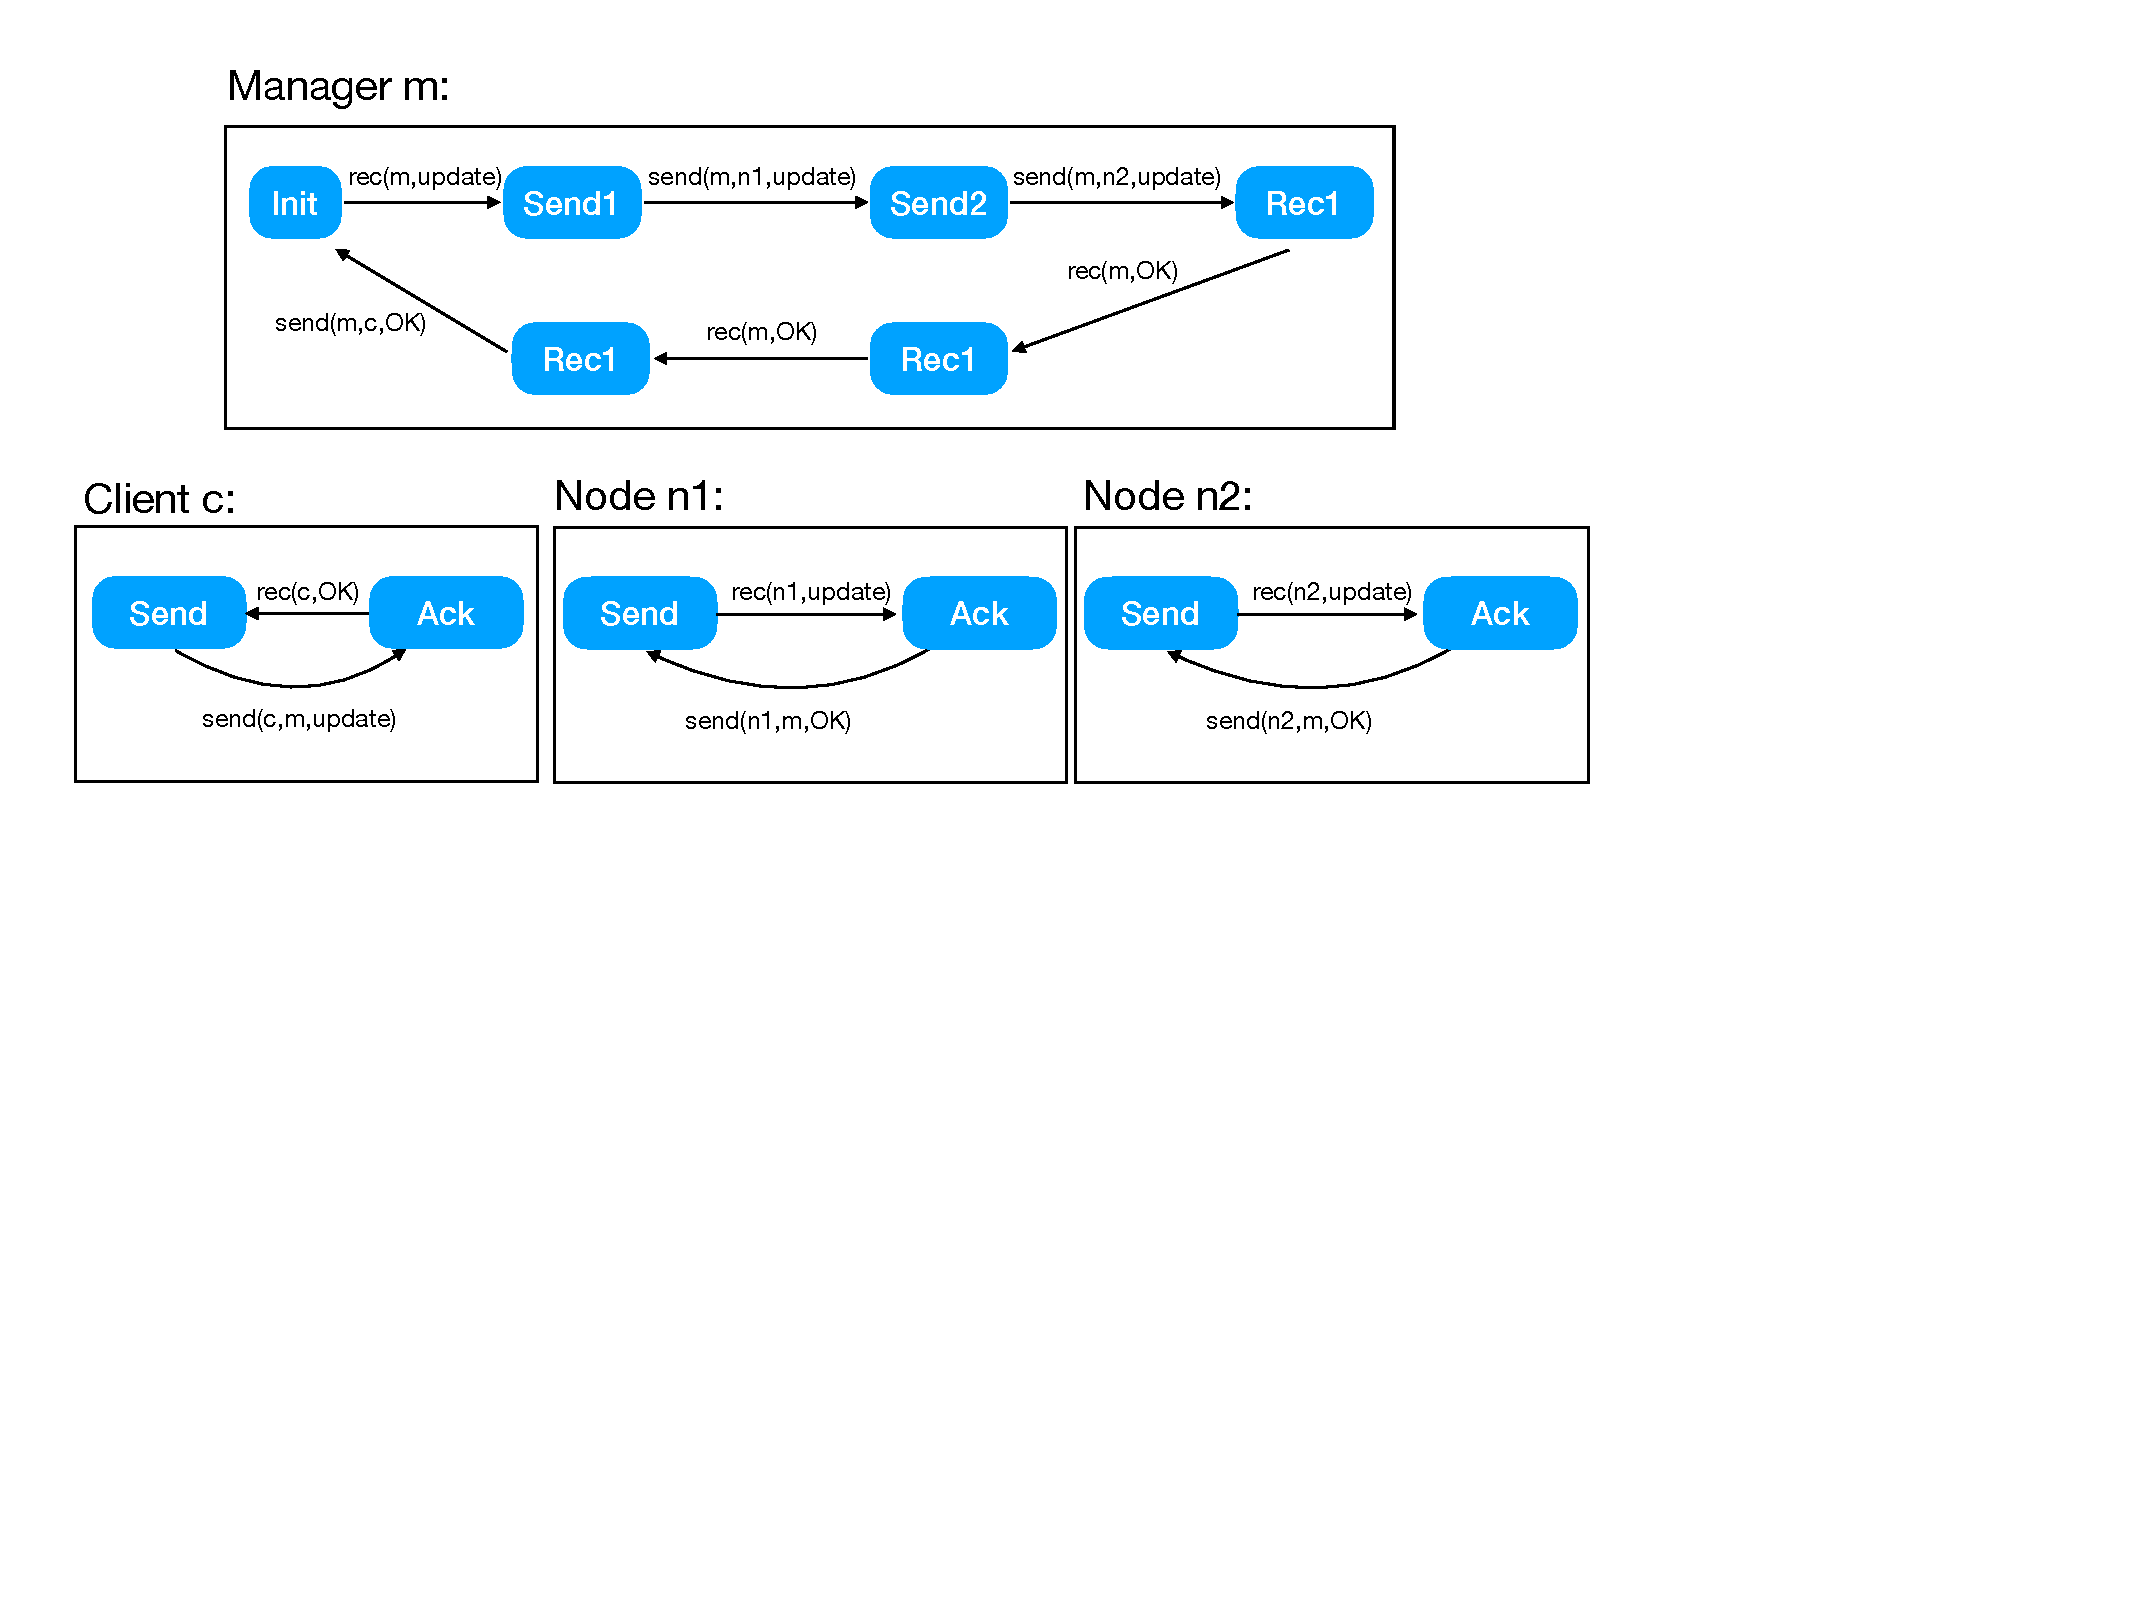
\includegraphics[width=10cm]{commit.pdf}
\caption{A distributed commit protocol. Each process is represented by a labeled transition system, where the transitions are labeled by send and receive actions. For instance, $\senda{\sf{c},\sf{m},\sf{update}}$ represents a send from the process $\sf{c}$ (the client) to the process $\sf{m}$ (the manager) with payload $\sf{update}$. Similarly, $\reca{c,\sf{OK}}$ represents the fact that the process $\sf{c}$ receives a message 
$\sf{OK}$.}
\label{fig:commit}
\end{figure}

\begin{figure}[t]
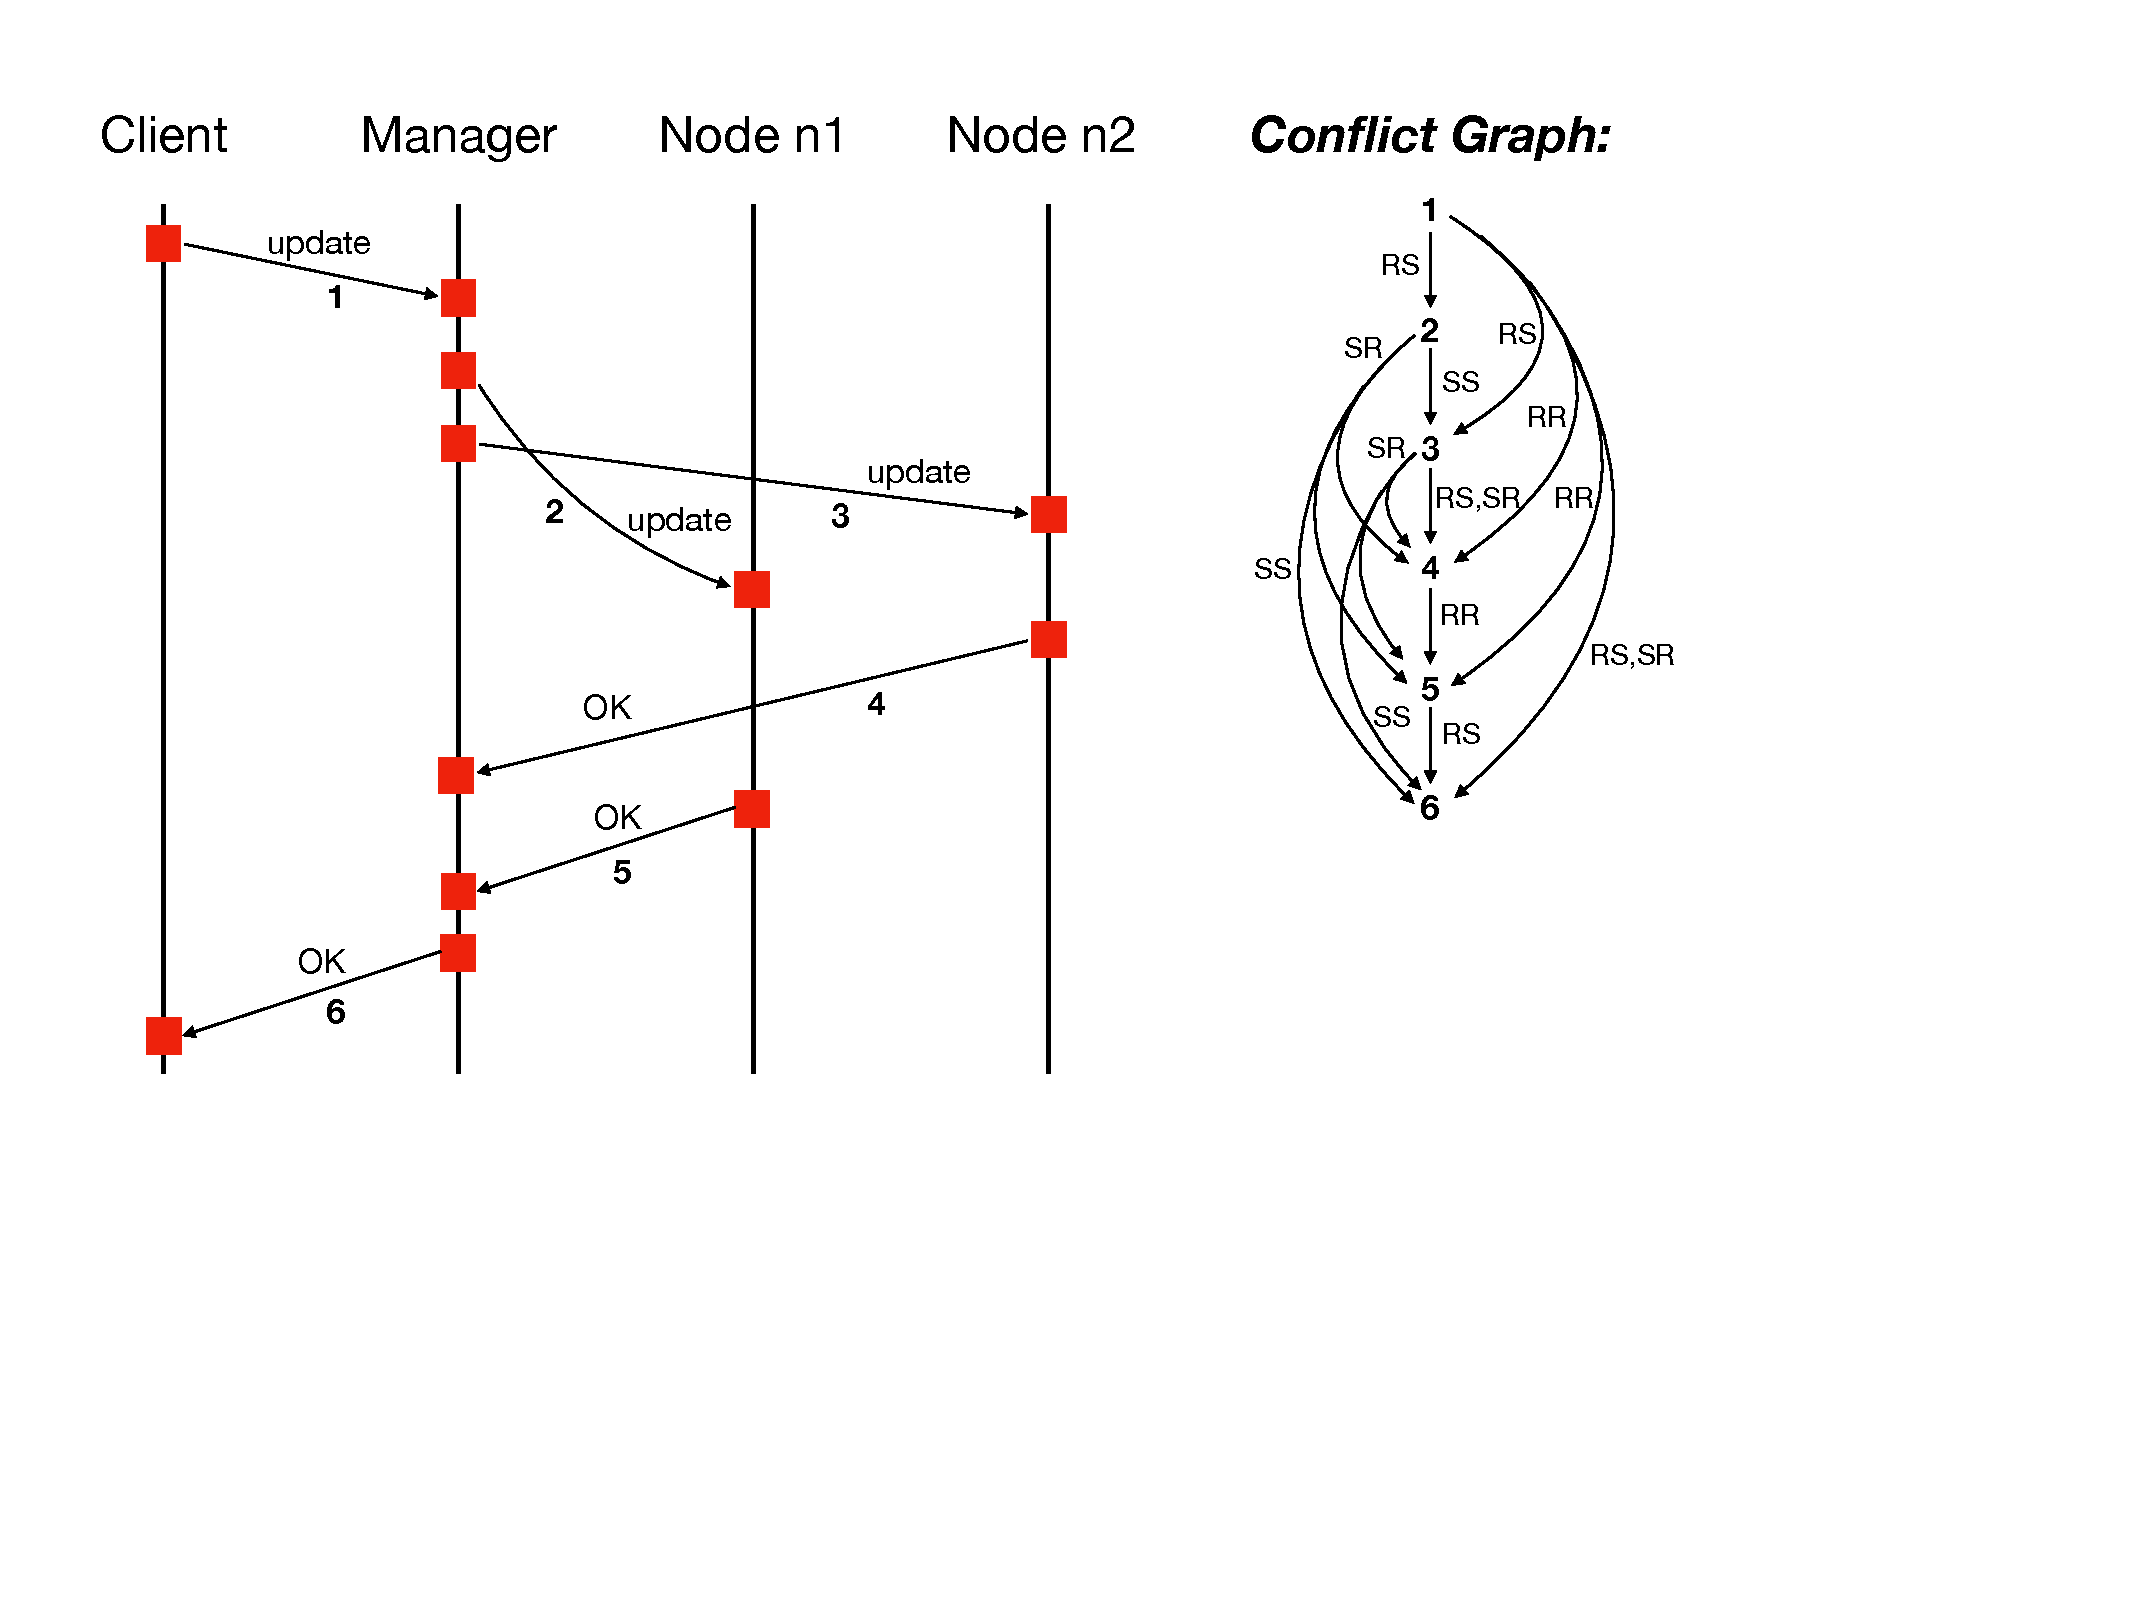
\includegraphics[width=7cm]{MSC-commit.pdf}
\caption{An execution of the distributed commit protocol and its conflict graph.}
\label{fig:commit-exec}
\end{figure}

Now, it can be observed that in the commit protocol message buffers are bounded in all the possible computations. This is in general not the case for 1-synchronizable systems. It might be the case indeed that there are asynchronous computations where buffers may have an arbitrarily size, that are however all equivalent to synchronous computations. This is illustrated for instance by a (family of) computations shown in Figure~\ref{fig:elevator-exec1} of the elevator system shown in Figure \ref{fig:elevator} (a simplified version of the system described in~\cite{DBLP:conf/pldi/DesaiGJQRZ13}).  In this execution, the user keeps sending requests for closing the door, which generates an unbounded sequence of messages in the entry buffer of the elevator process. However, these computations are synchronizable since it is possible to consider the synchronous computation where the elevator receives immediately the messages sent by the client. The fact that this is possible is witnessed by the acyclicity of the conflict graph of this computation (shown on the right of the same figure). It can be checked that the elevator system shown in Figure \ref{fig:elevator} is a 1-synchronous system (without the dashed edge). 

Consider now a slightly different version of the elevator system where the transition from {\sf Stopping2} to {\sf Opening2} is moved to target {\sf Opening1} instead of {\sf Opening2} (see the dashed transition in Figure \ref{fig:elevator}). It can be seen that this version has the same state space as the previous one. Indeed, moving that transition from {\sf Stopping2} to {\sf Opening1} gives the possibility to {\sf Elevator} to send a message open to {\sf Door}, but the latter can only be between {\sf StopDoor} and {\sf ResetDoor} at this point, and therefore it can (maybe after sending {\sf doorStoped} and {\sf doorOpened}) receive at state {\sf ResetDoor} the message {\sf open} and stay in the same state. However, this version of the system is not 1-synchronizable as it is shown in Figure \ref{fig:elevator-exec2}: Suppose that {\sf Door} is at state {\sf StopDoor}, and that {\sf Elevator} is at state {\sf Stopping2}. Then, {\sf Door} can send a message {\sf doorStoped} and move to the state {\sf OpenDoor}. Next, {\sf Elevator} can receive that message and move to state {\sf Opening1}. At this point, {\sf Elevator} and {\sf Door} can only exchange messages: message {\sf doorOpened} from {\sf Door} to {\sf Elevator} and message {\sf open} from {\sf Elevator} to {\sf Door}. The conflict graph of this execution, shown on the right of Figure \ref{fig:elevator-exec2}, contains a cycle of size 2 between the two matching pairs of send-receive actions involved in the exchange interaction. 

\begin{figure}[t]
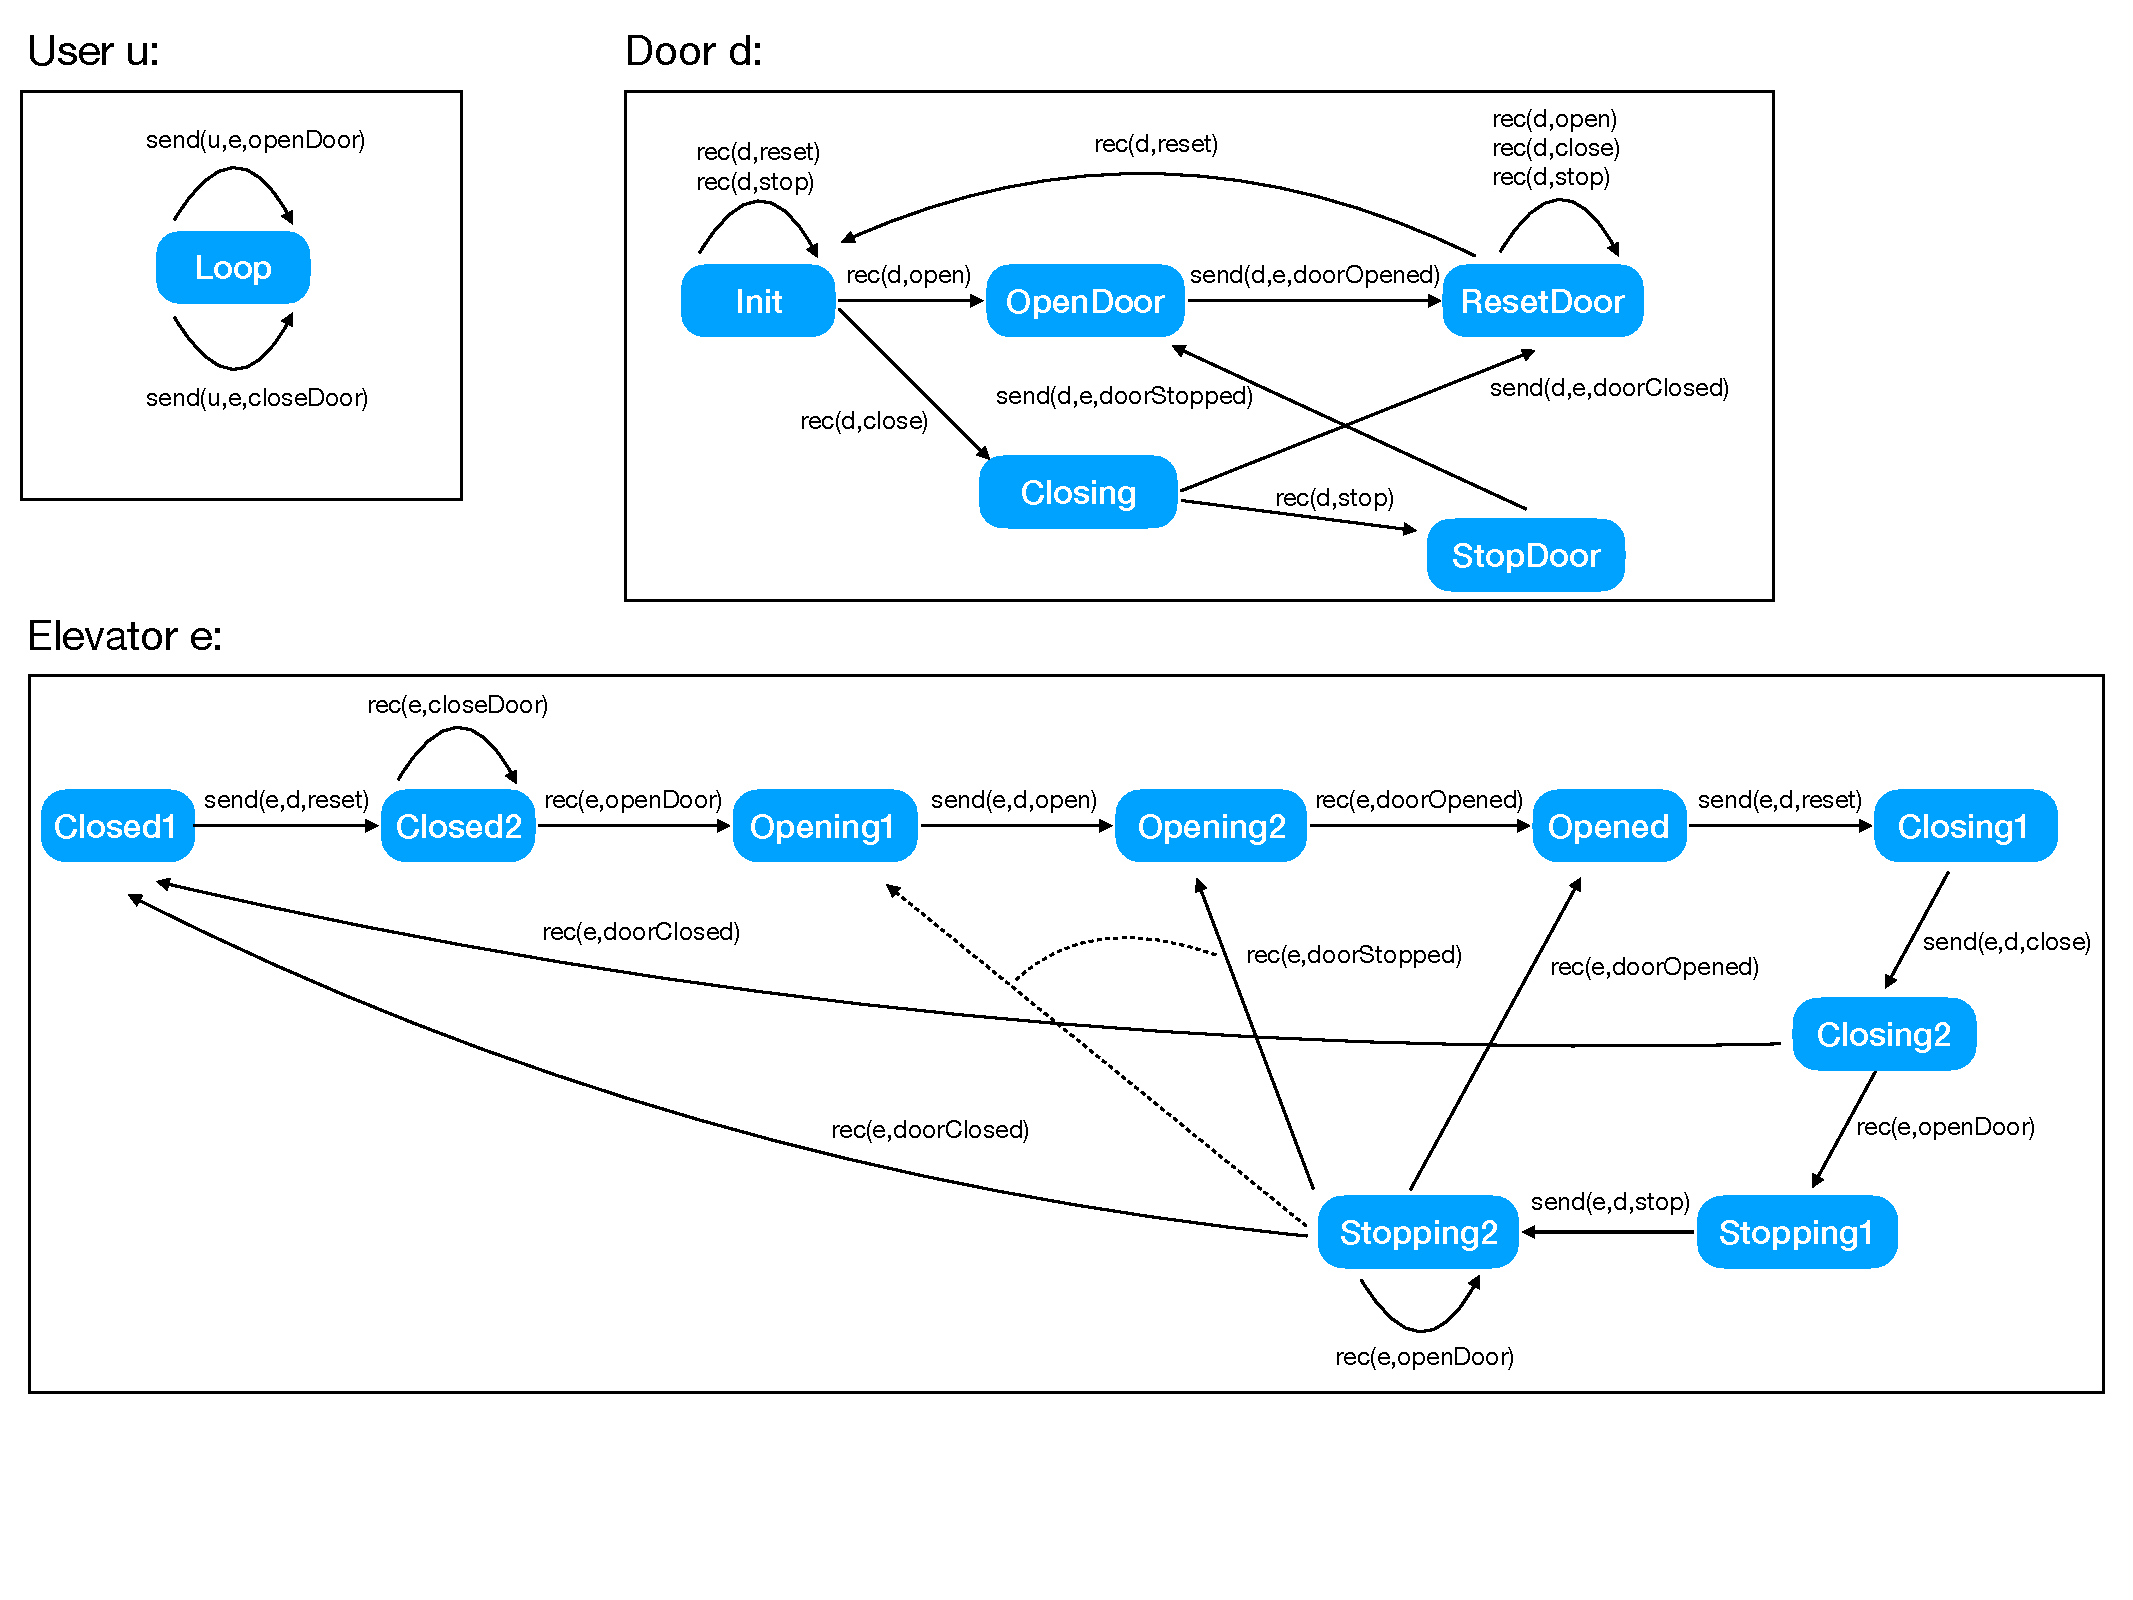
\includegraphics[width=13cm]{elevator.pdf}
\caption{The Elevator example}
\label{fig:elevator}
\end{figure}

\begin{figure}[t]
\begin{subfigure}[t]{6cm}
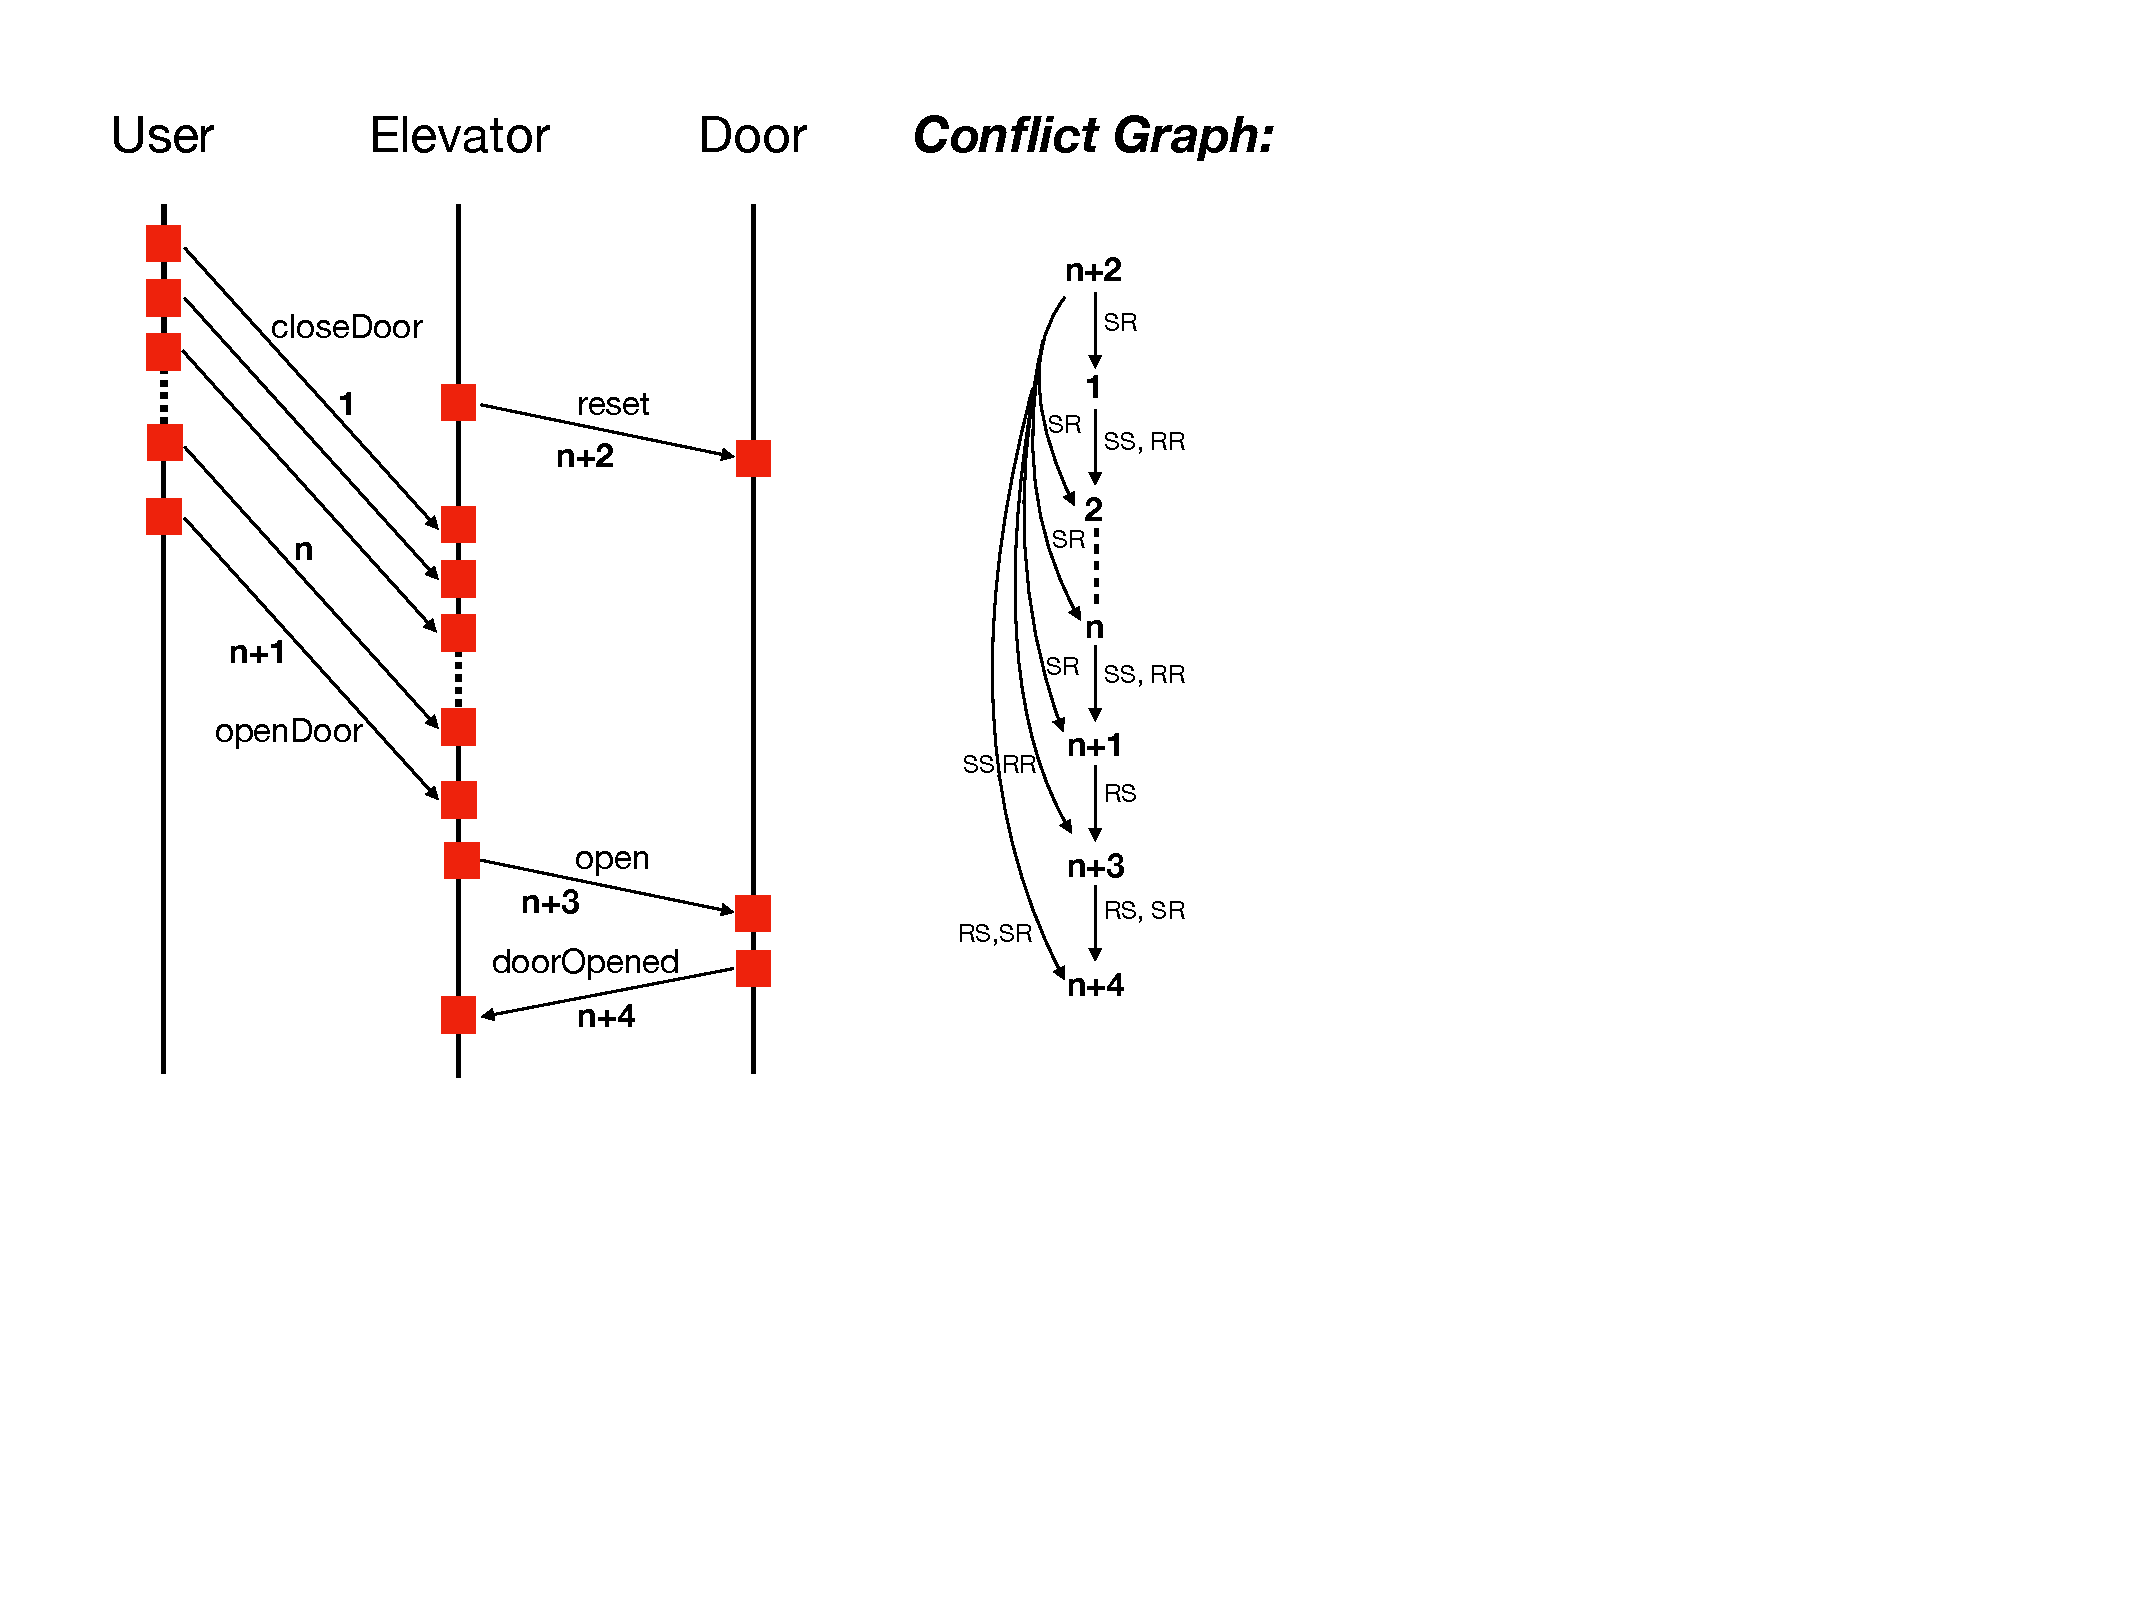
\includegraphics[width=6cm]{MSC-elevator1.pdf}
\caption{A $1$-synchronizable execution.}
\label{fig:elevator-exec1}
\end{subfigure}
\hspace{1cm}
\begin{subfigure}[t]{5cm}
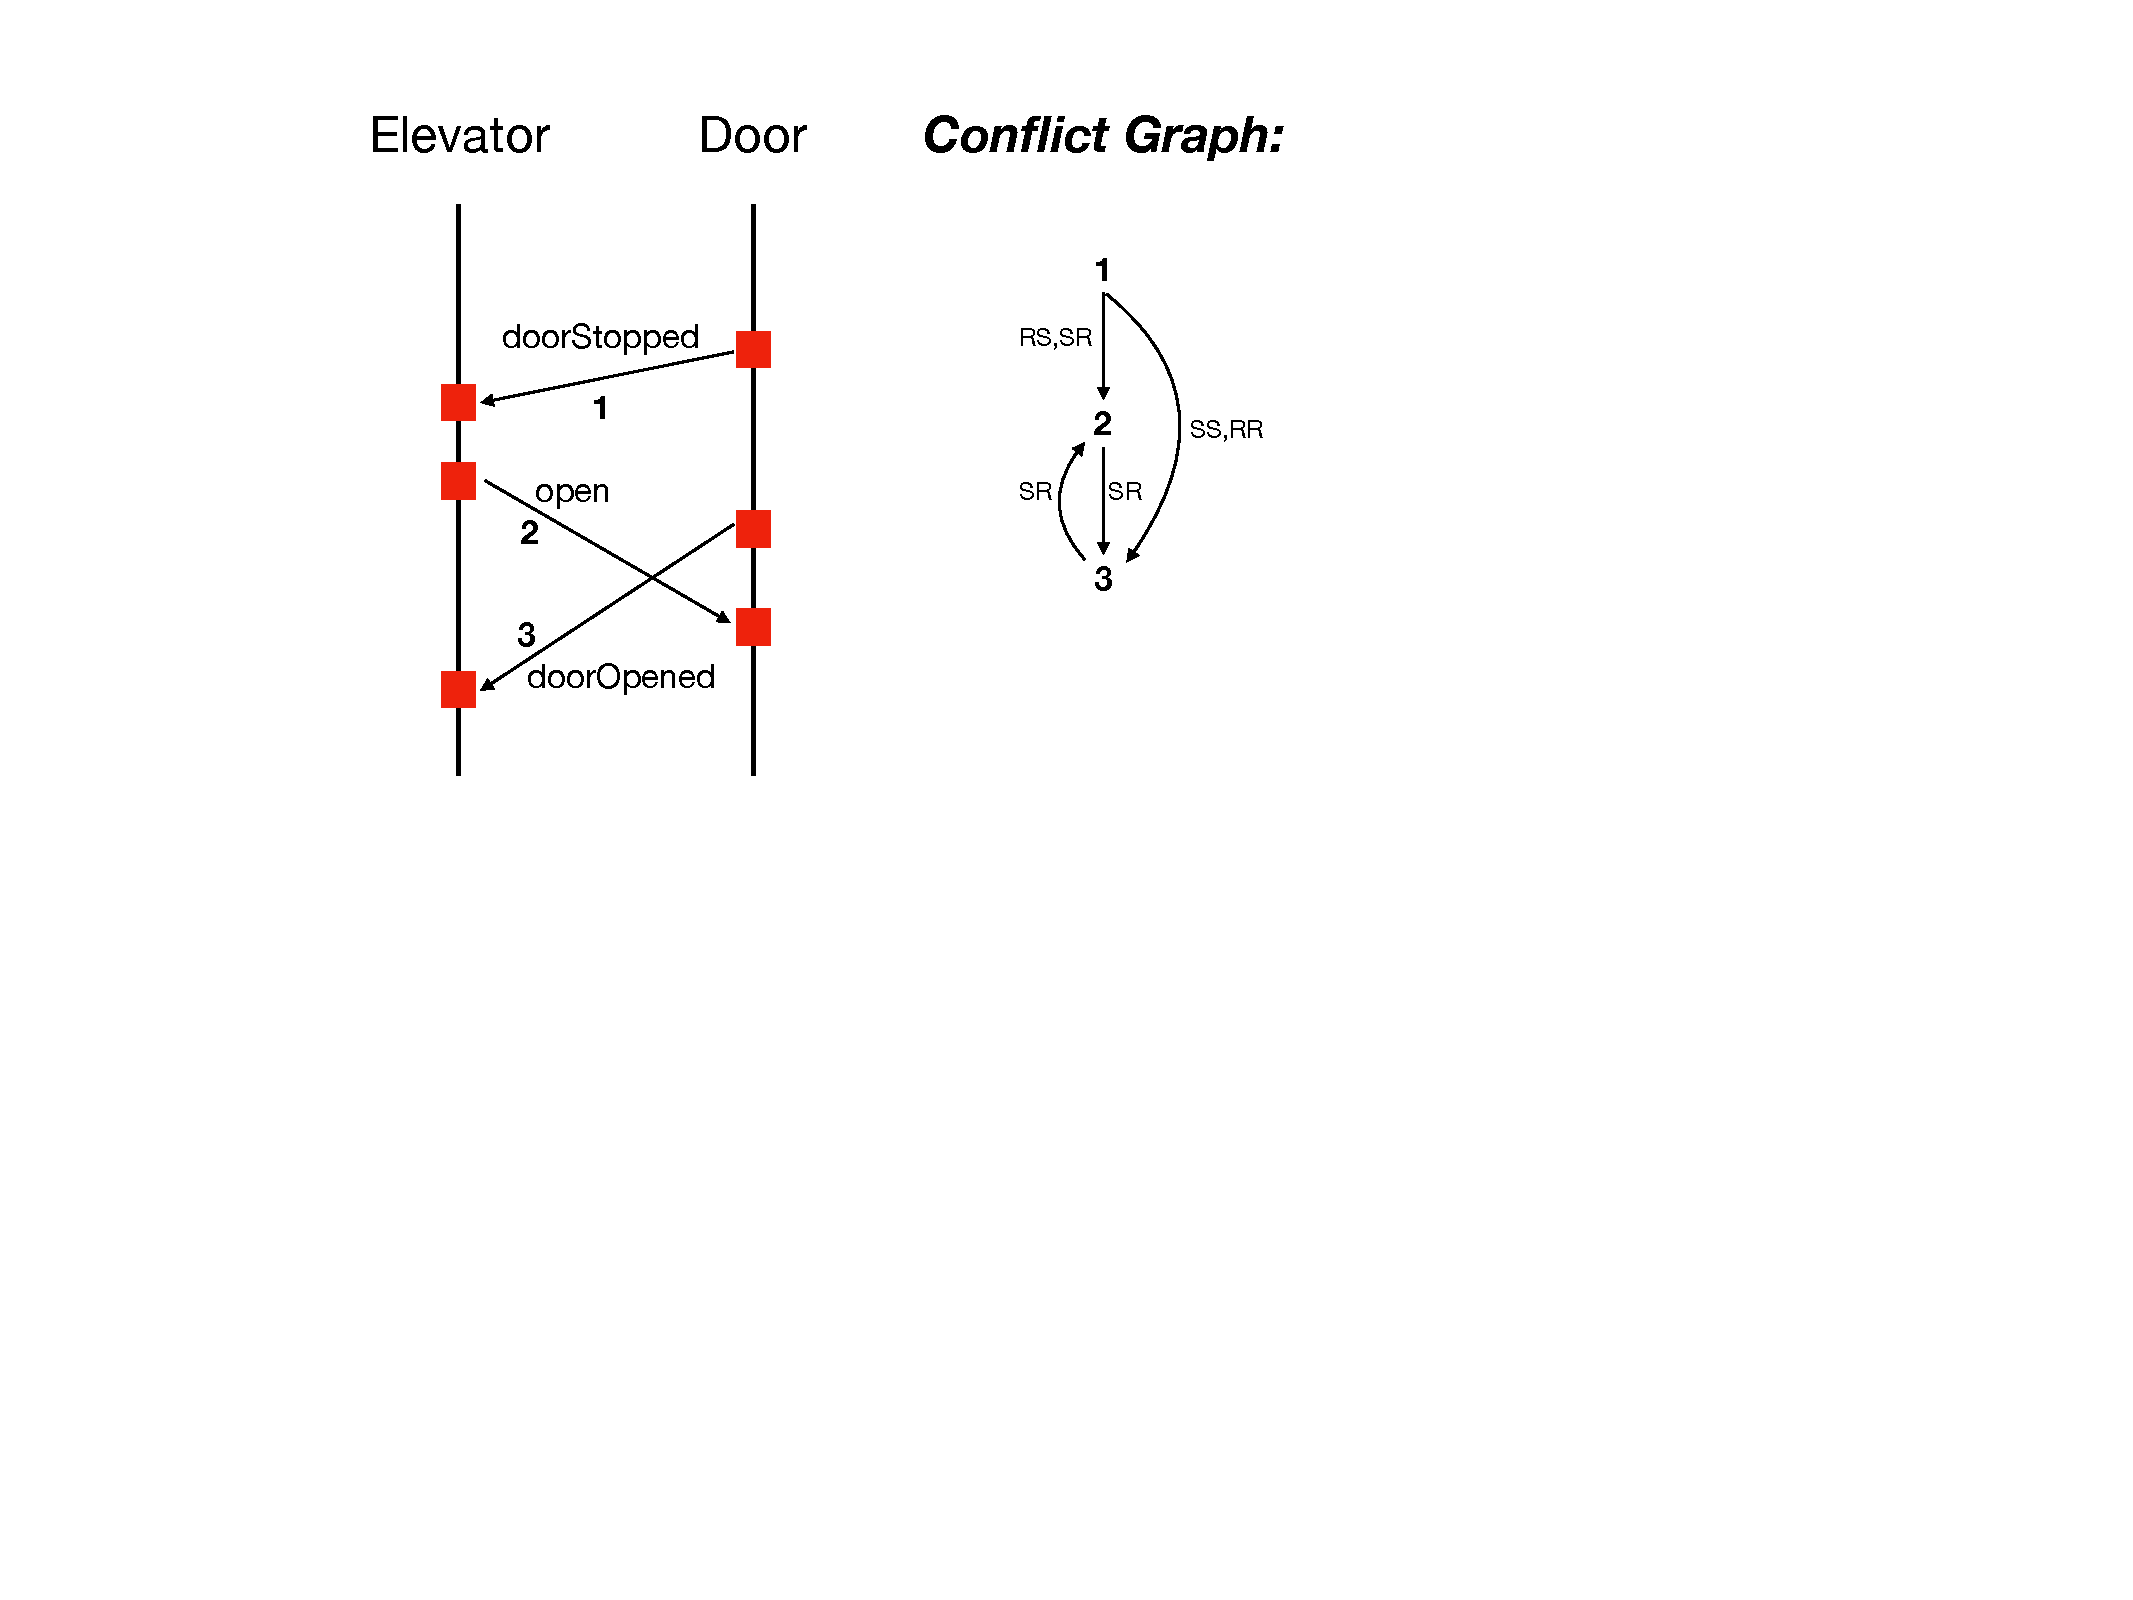
\includegraphics[width=5cm]{MSC-elevator2.pdf}
\caption{A computation with a 2-exchange.}
\label{fig:elevator-exec2}
\end{subfigure}
\caption{Executions of the Elevator.}
\label{fig:elevator-exec}
\end{figure}

%\begin{figure}
%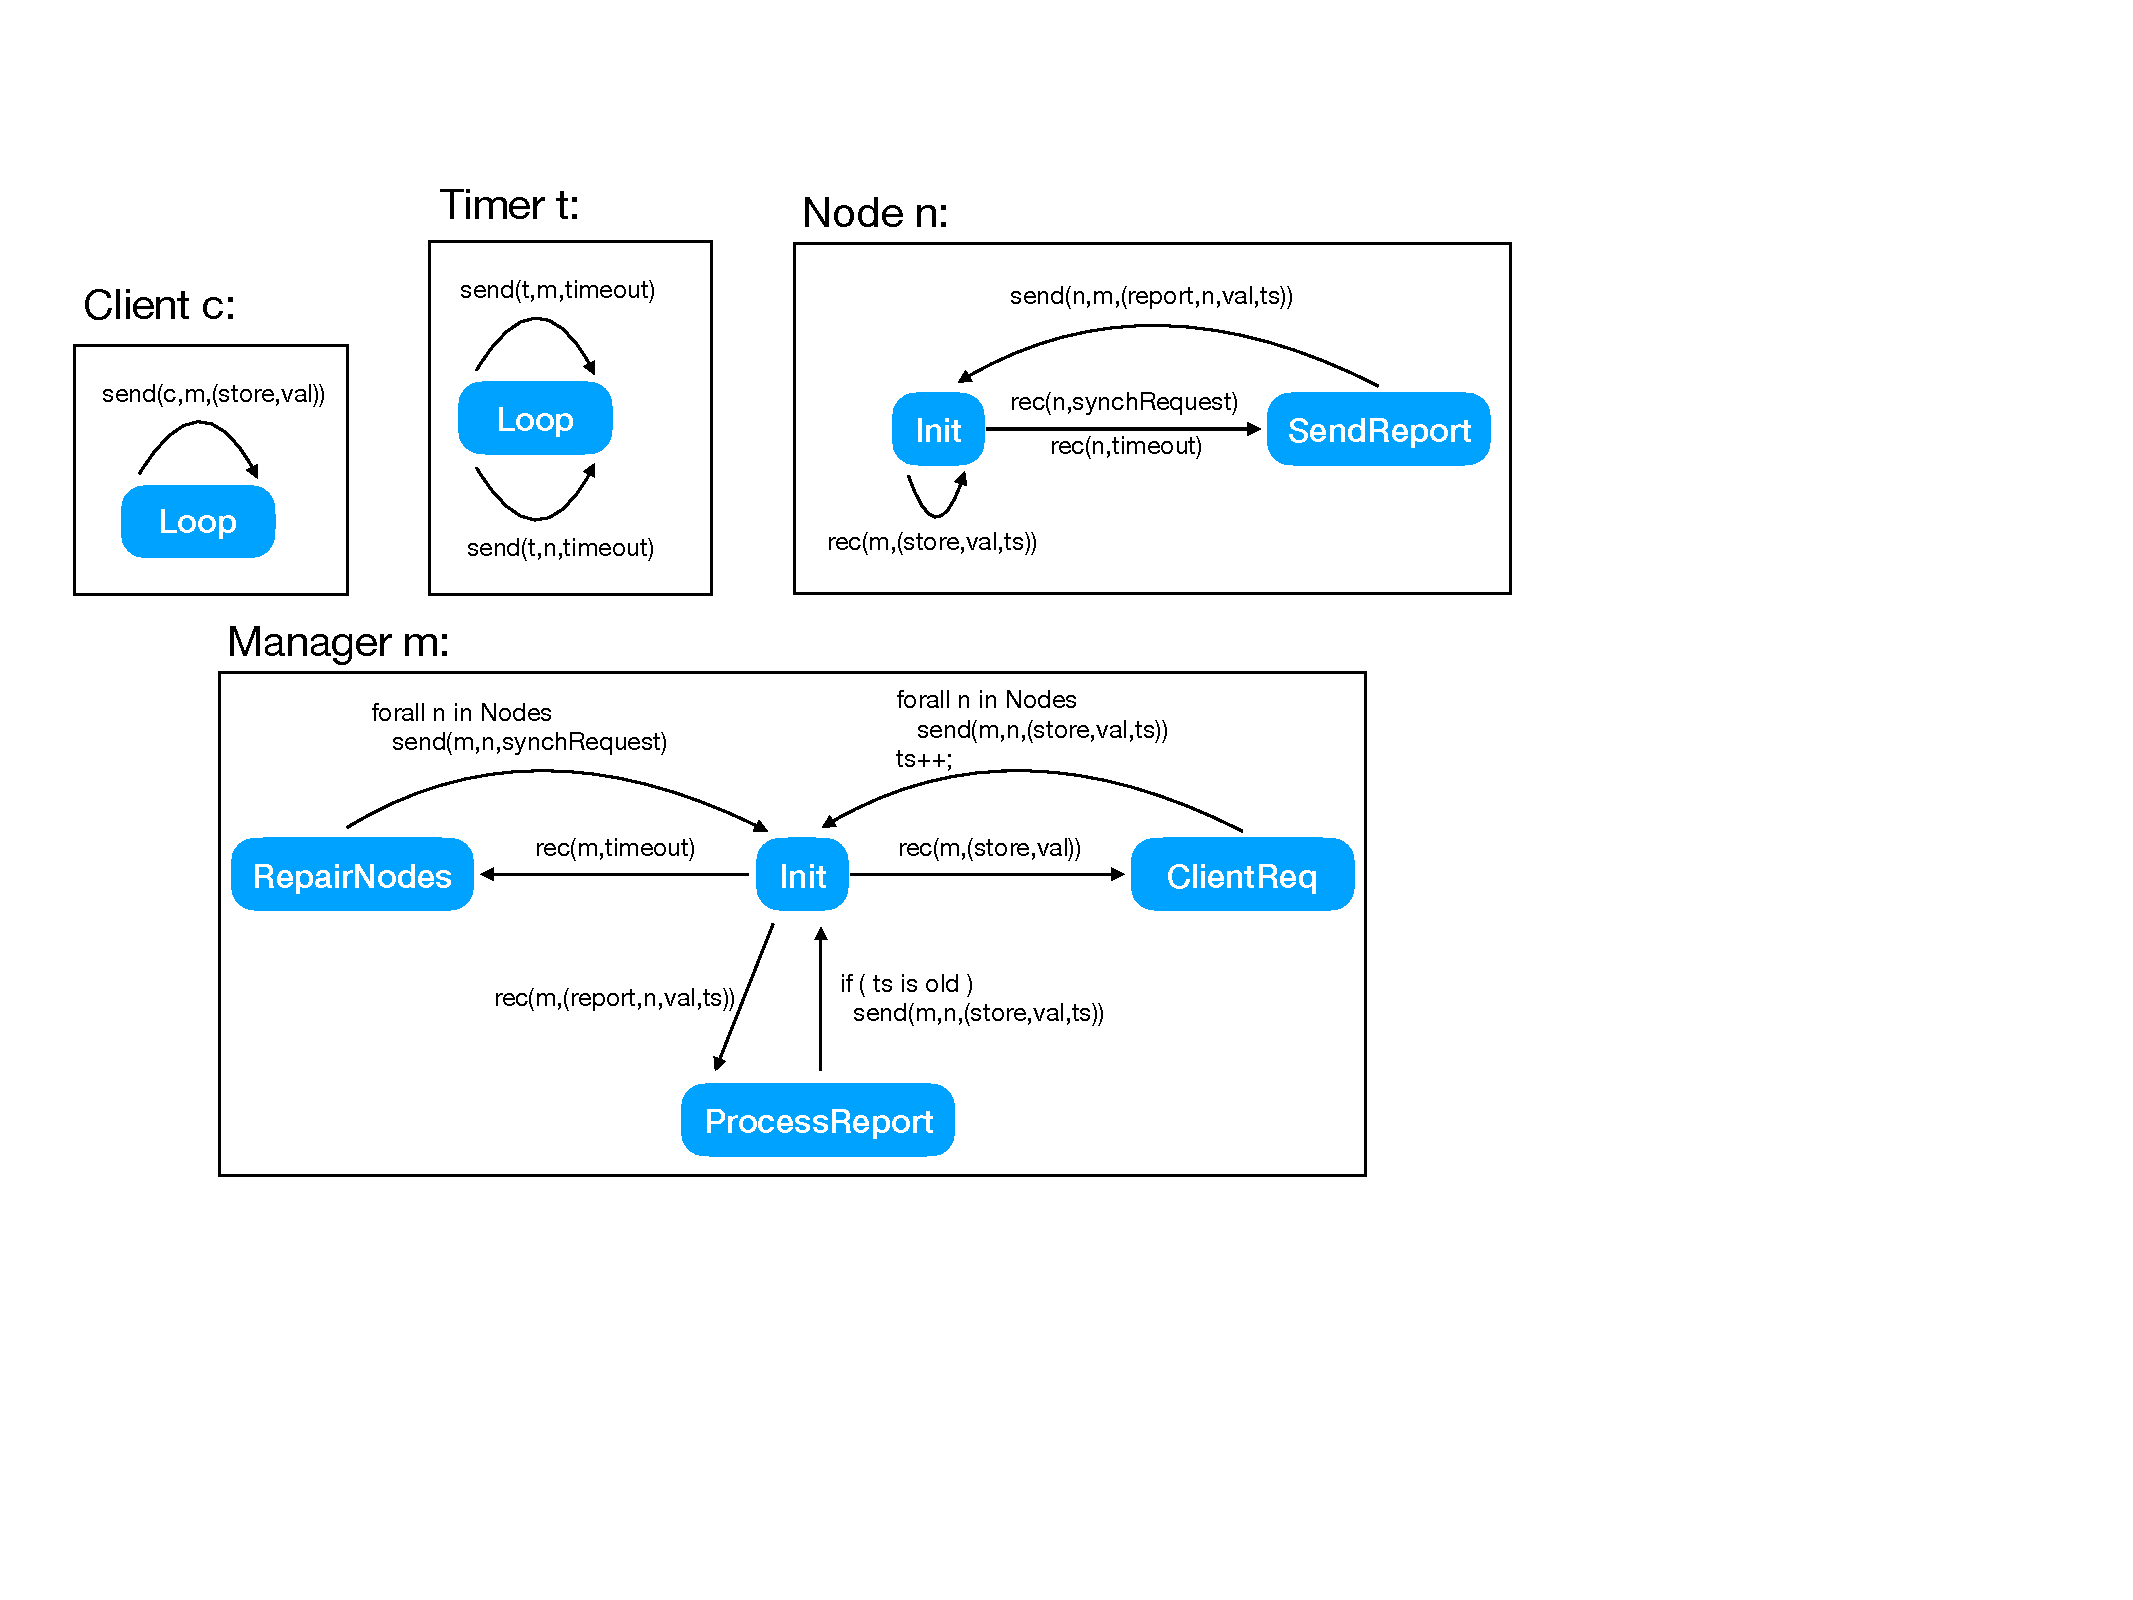
\includegraphics[width=10cm]{replication.pdf}
%\caption{A replication storage protocol}
%\label{fig:replication}
%\end{figure}
%
%\begin{figure}
%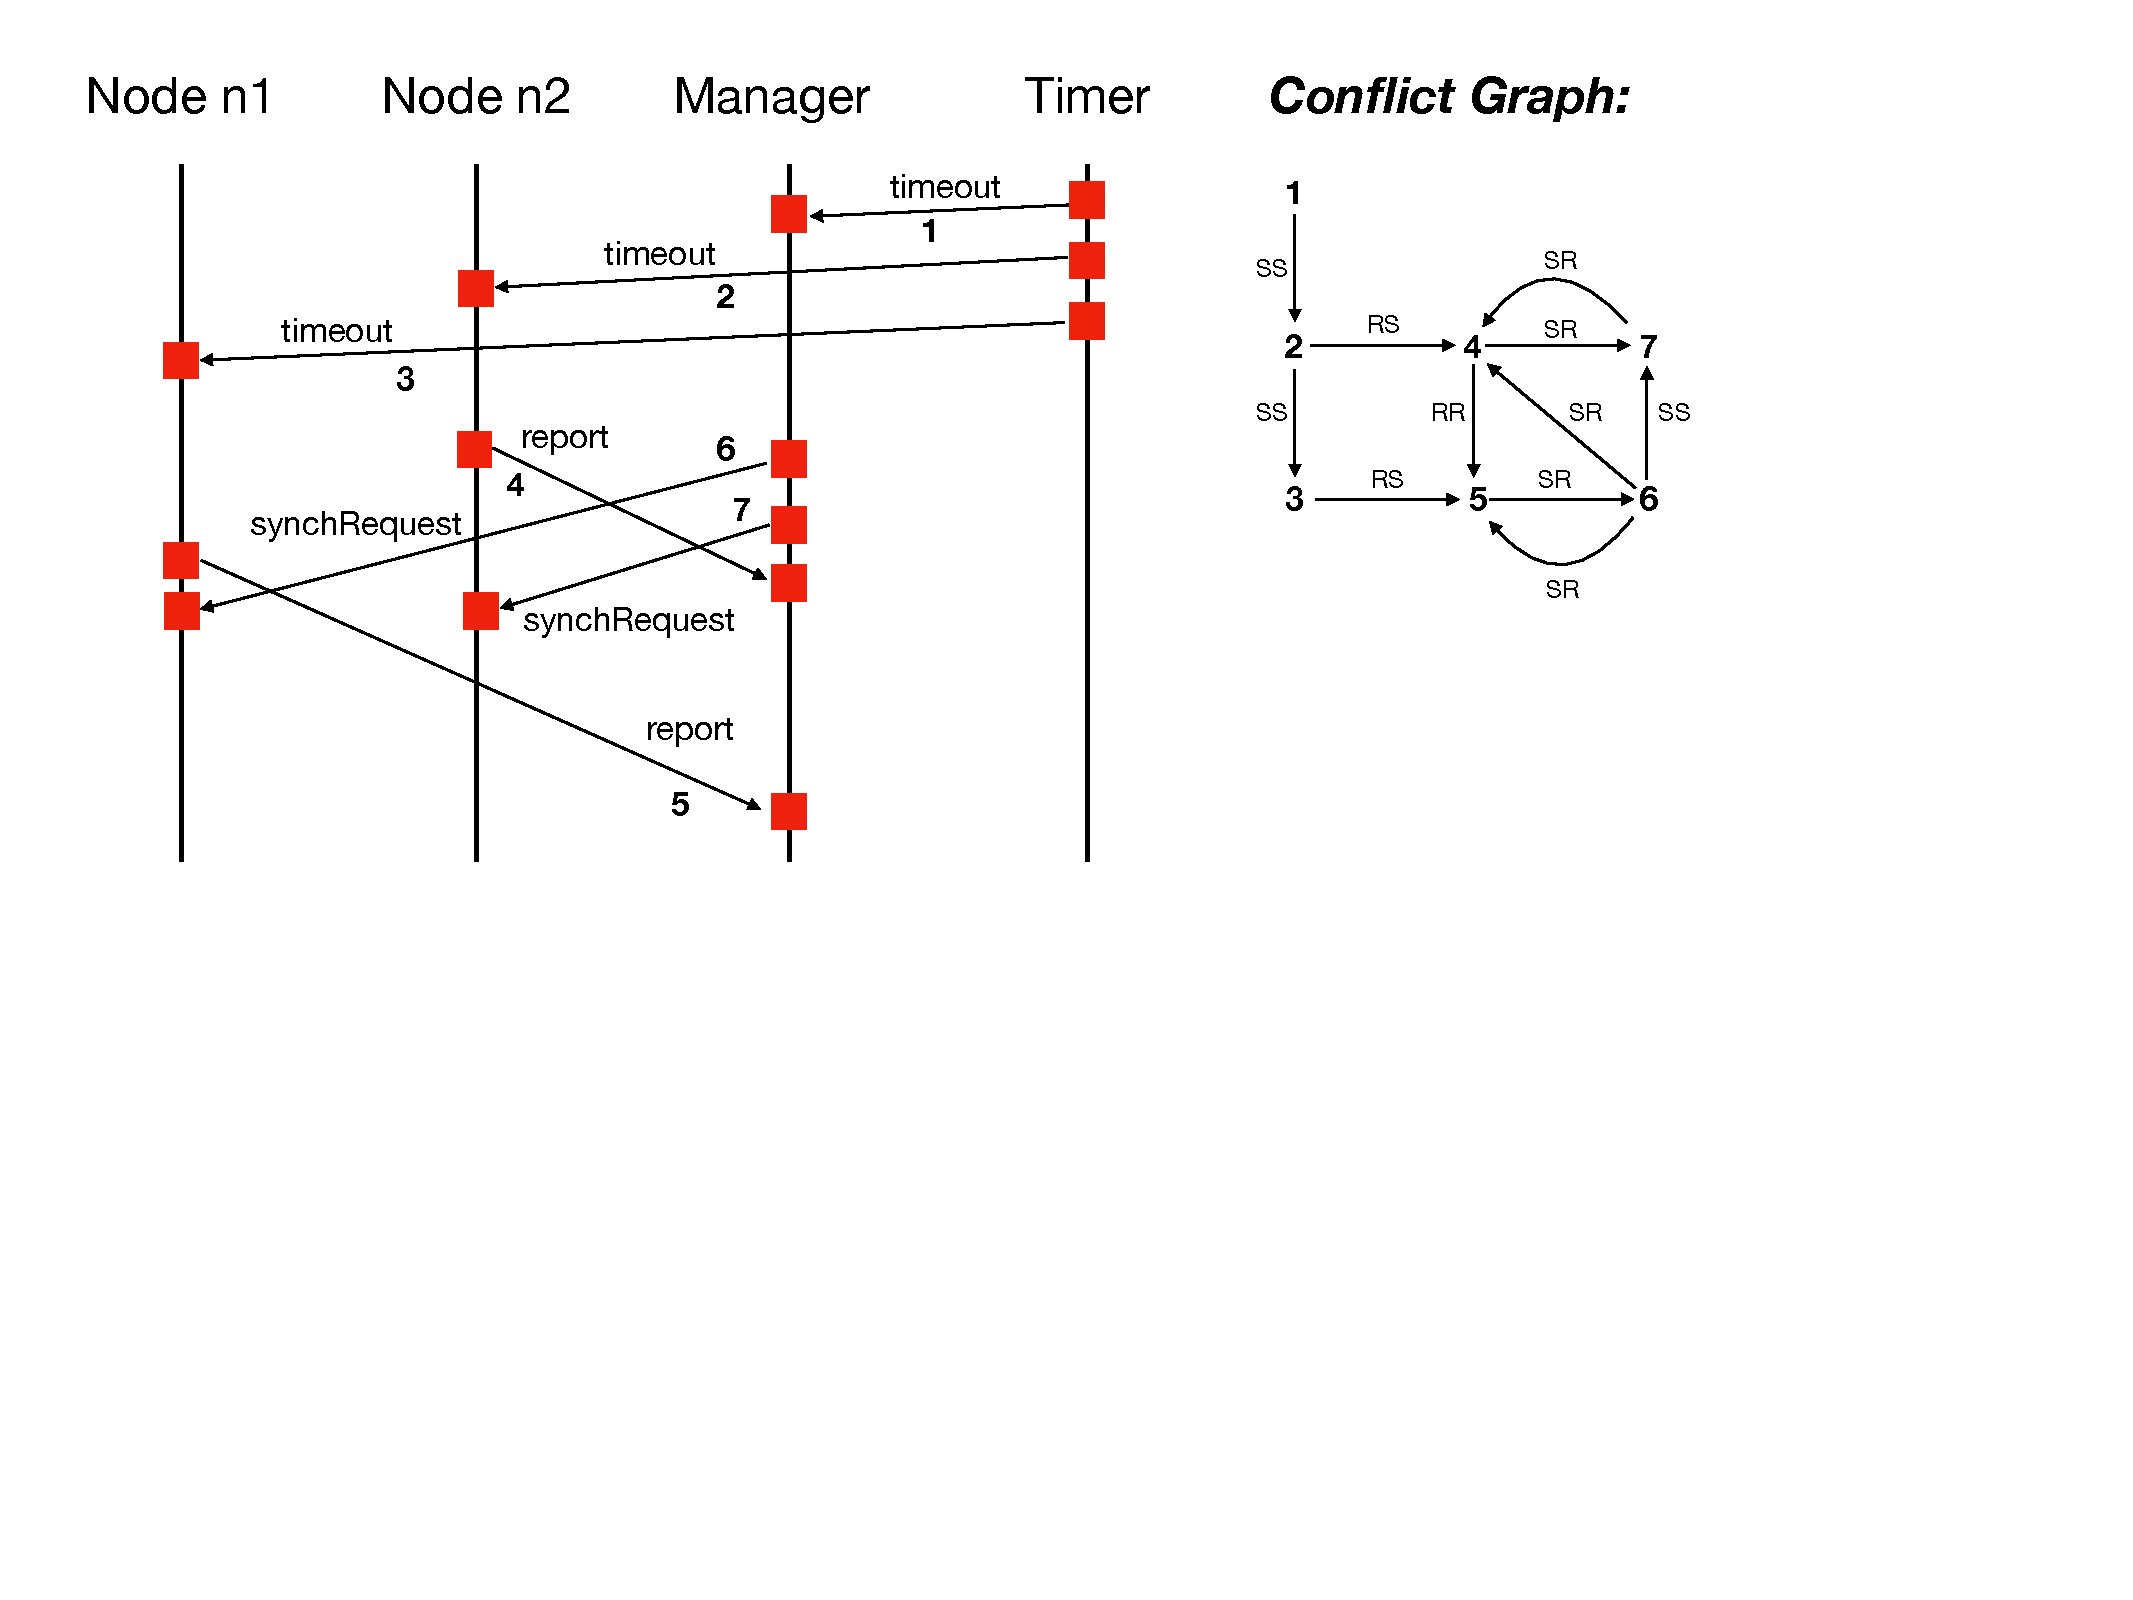
\includegraphics[width=7cm]{MSC-storage.pdf}
%\caption{An execution of the replication storage protocol and its conflict graph.}
%\label{fig:replic-exec}
%\end{figure}


Finally, we present an example illustrating the fact that exchanges can involve not only 2 processes but several ones, maybe all the processes of a system. Figure \ref{fig:replication} shows a replication storage protocol. A client can send update requests to the manager who is in charge of maintaining several storage replicas on different nodes. When the manager receives an update request from the client, it forwards this message to all the nodes. However, since messages can be delayed, the information in the nodes can be different at various points in time. Then, a mechanism is used to force regularly synchronization between the data versions stored in the different nodes. This mechanism is based on (1) using time-stamps for each message that is sent  by the manager to the nodes, and (2) a timer that triggers synchronizations: the timer can send timeout messages to either the manager or to the nodes. When a node receives such a timeout message, it sends a report to the manager with its current data value, and when the manager receives the timeout message, it sends to all nodes a message requesting a synchronization. When a node receives the synchronization request, it sends to the manager a report with its last value. After each reception of a report from a node, the manager checks if the received value is up-to-date using its time-stamp, and if not, it sends the most recent value to the node. Now, since the nodes and the manager may all receive timeout messages from the timer, nodes can start sending reports to the manager while the latter is already sending them synchronization requests. This leads to an exchange that may involve all the nodes, in addition to the manager. This situation is shown in Figure \ref{fig:replic-exec}. The conflict graph shown on the right of the figure contains a cycle of size 4, which is in this case the number of involved processes (two nodes and one manager), plus 1, which means that the considered computation is not 3-synchronizable. It can be checked that the system is actually 4-synchronizable. 

We have investigated other examples defined in the P language~\footnote{Available at \url{https://github.com/p-org}.}, e.g., an implementation of the German cache coherence protocol and an implementation of a device driver, and we have established manually and through testing that they are $k$-synchronizable~\footnote{For the testing part, we have checked on tens of thousands of executions generated through randomized testing, each execution with thousands of steps, that the corresponding conflict-graph satisfies the properties required for $k$-synchronizability.}. The value of $k$ is most of the times $1$ or $2$.

%\cite{PRuntime}

%\begin{figure}
%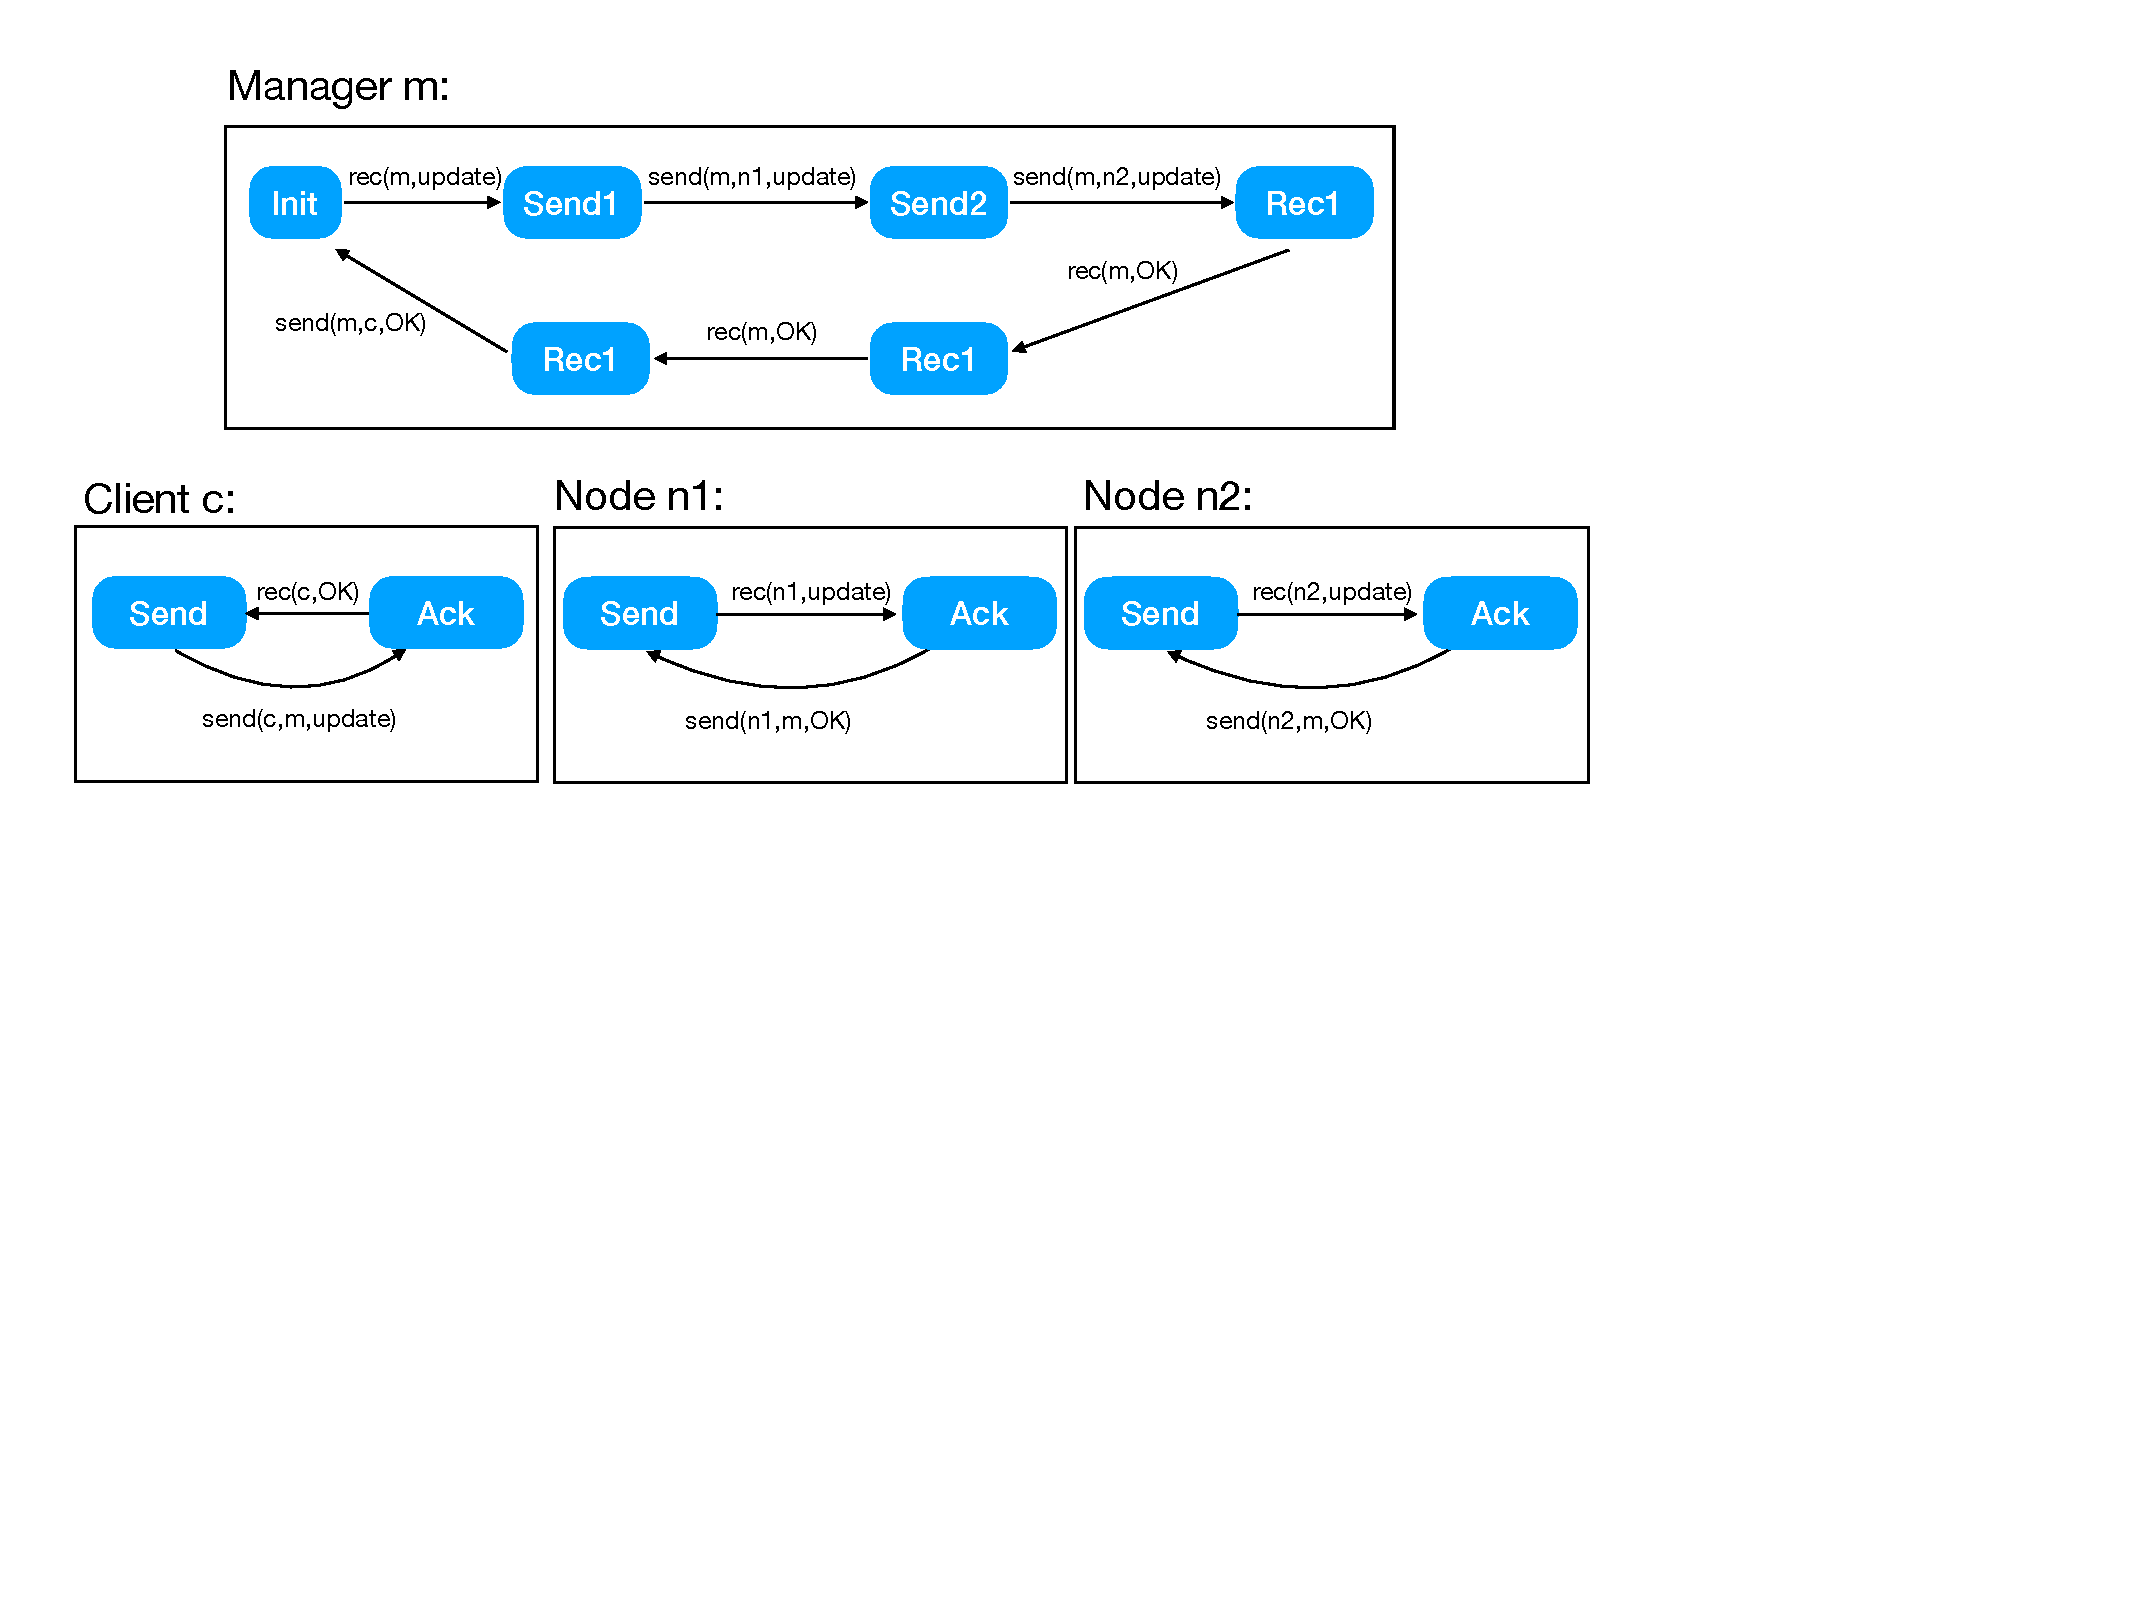
\includegraphics[width=10cm]{commit.pdf}
%\caption{A distributed commit protocol.}
%\label{fig:commit}
%\end{figure}
%
%\begin{figure}
%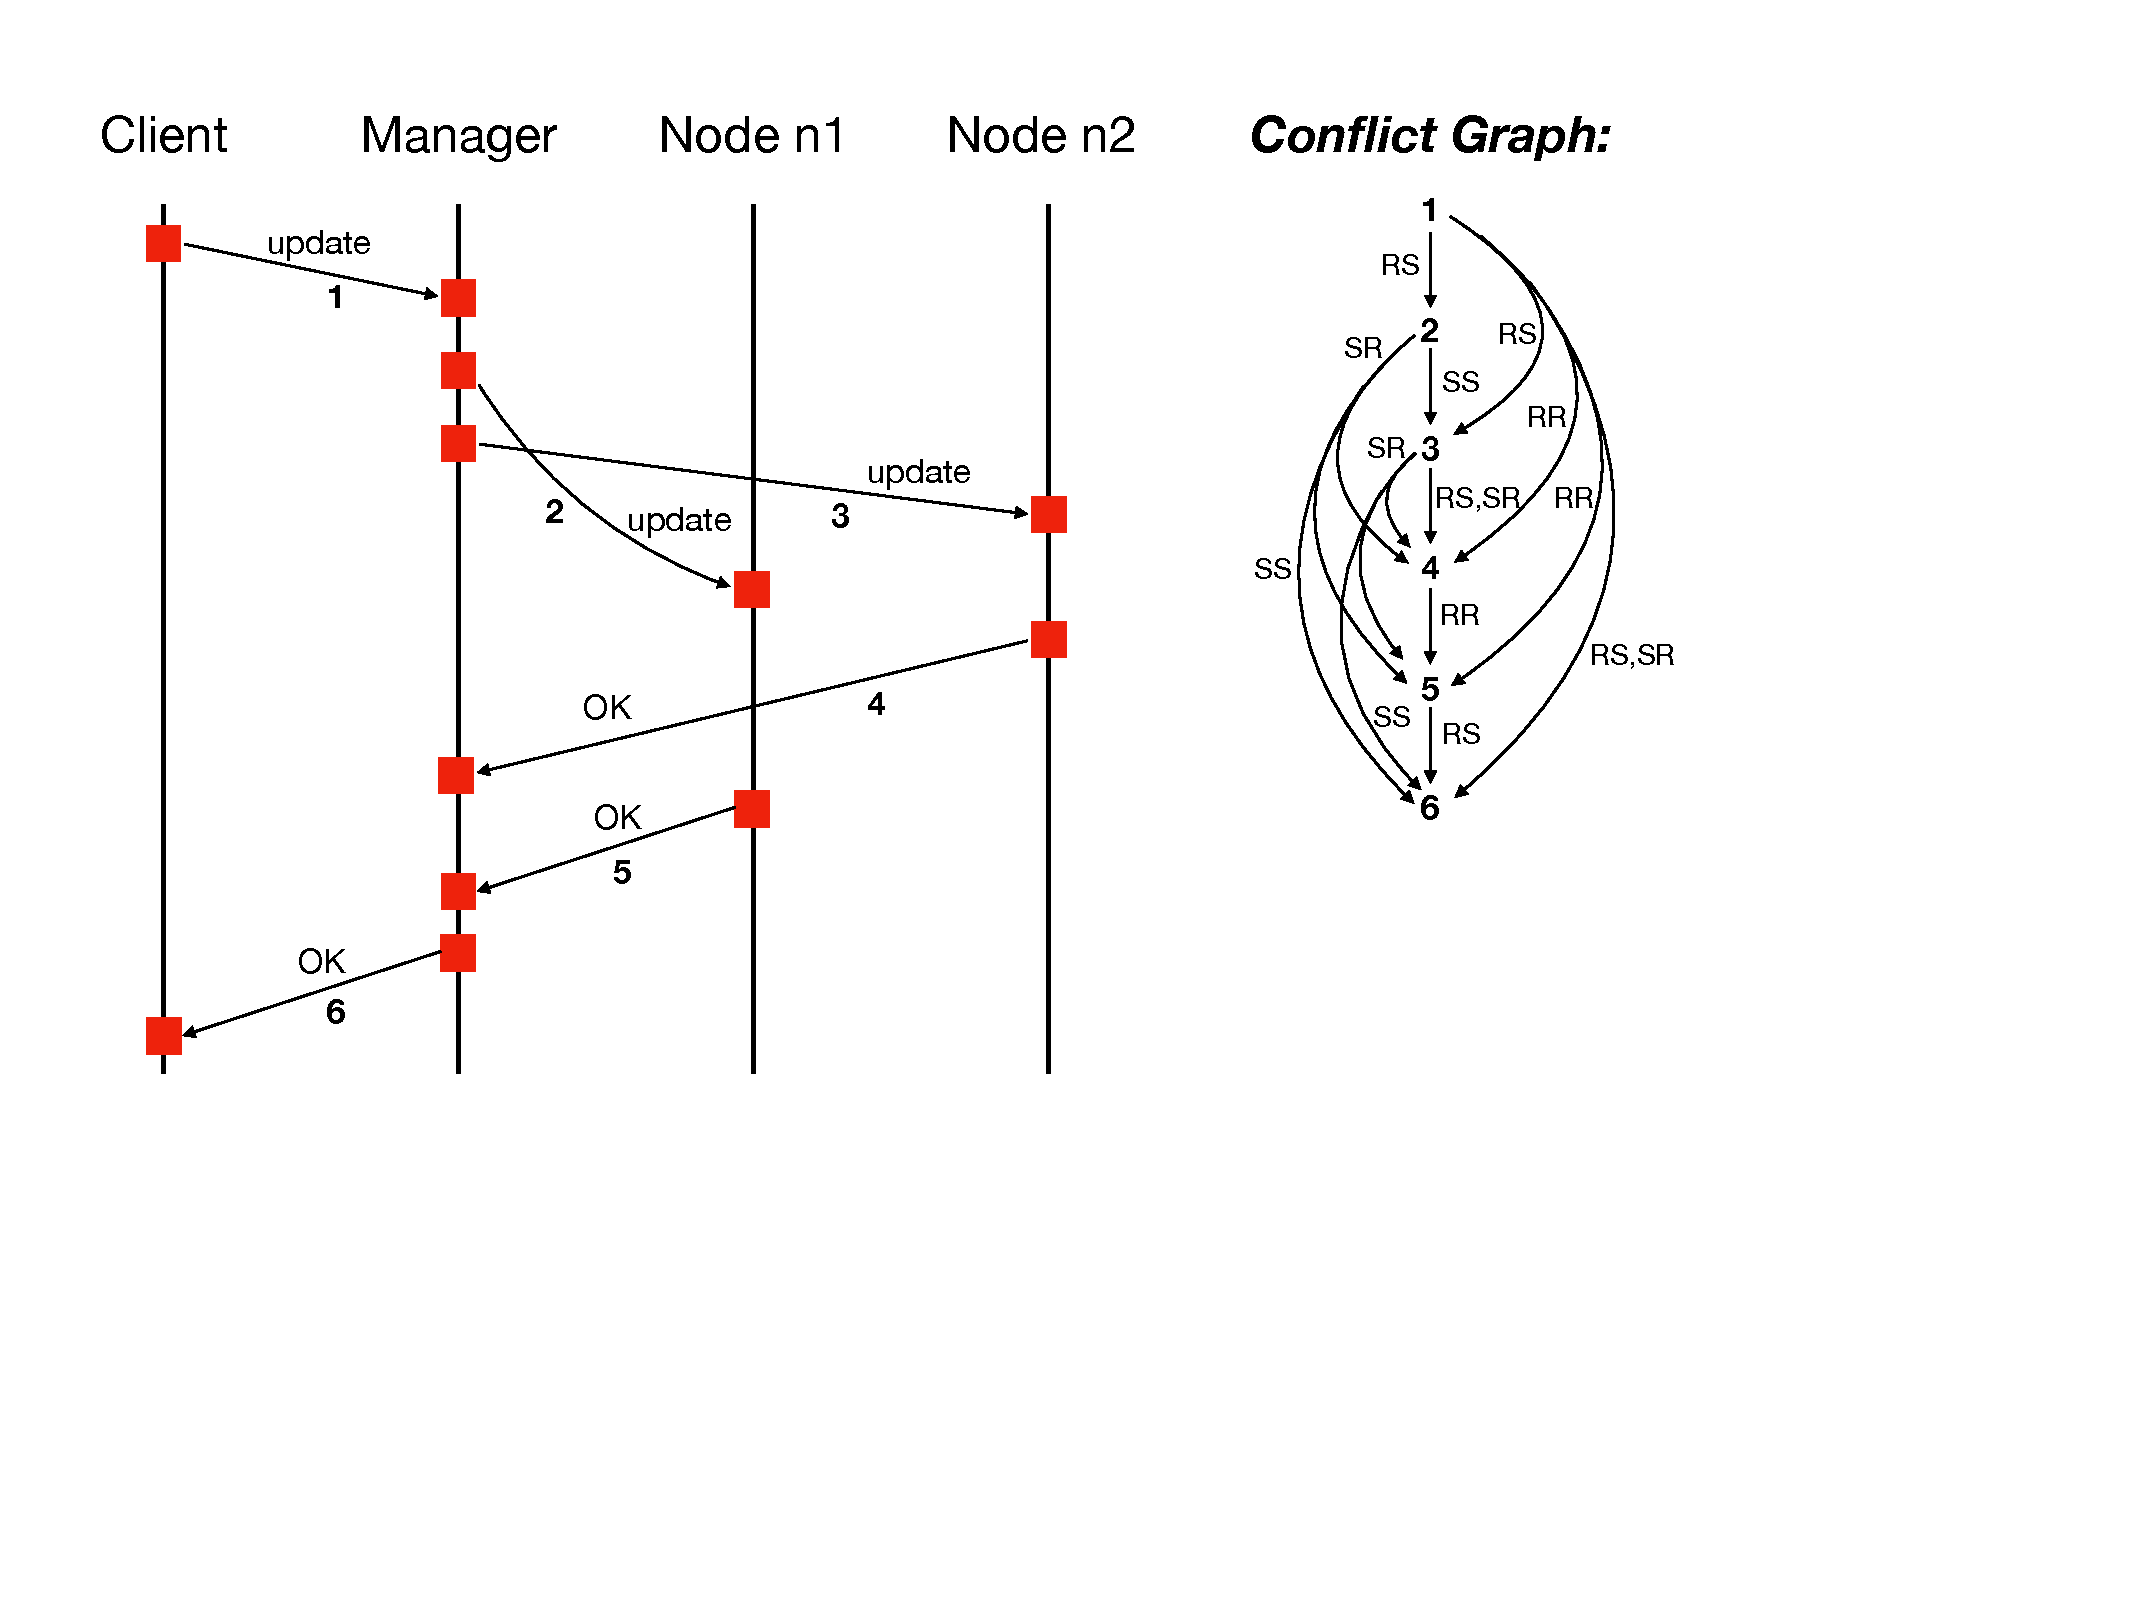
\includegraphics[width=7cm]{MSC-commit.pdf}
%\caption{An execution of the distributed commit protocol and its conflict graph.}
%\label{fig:commit-exec}
%\end{figure}

%\begin{figure}
%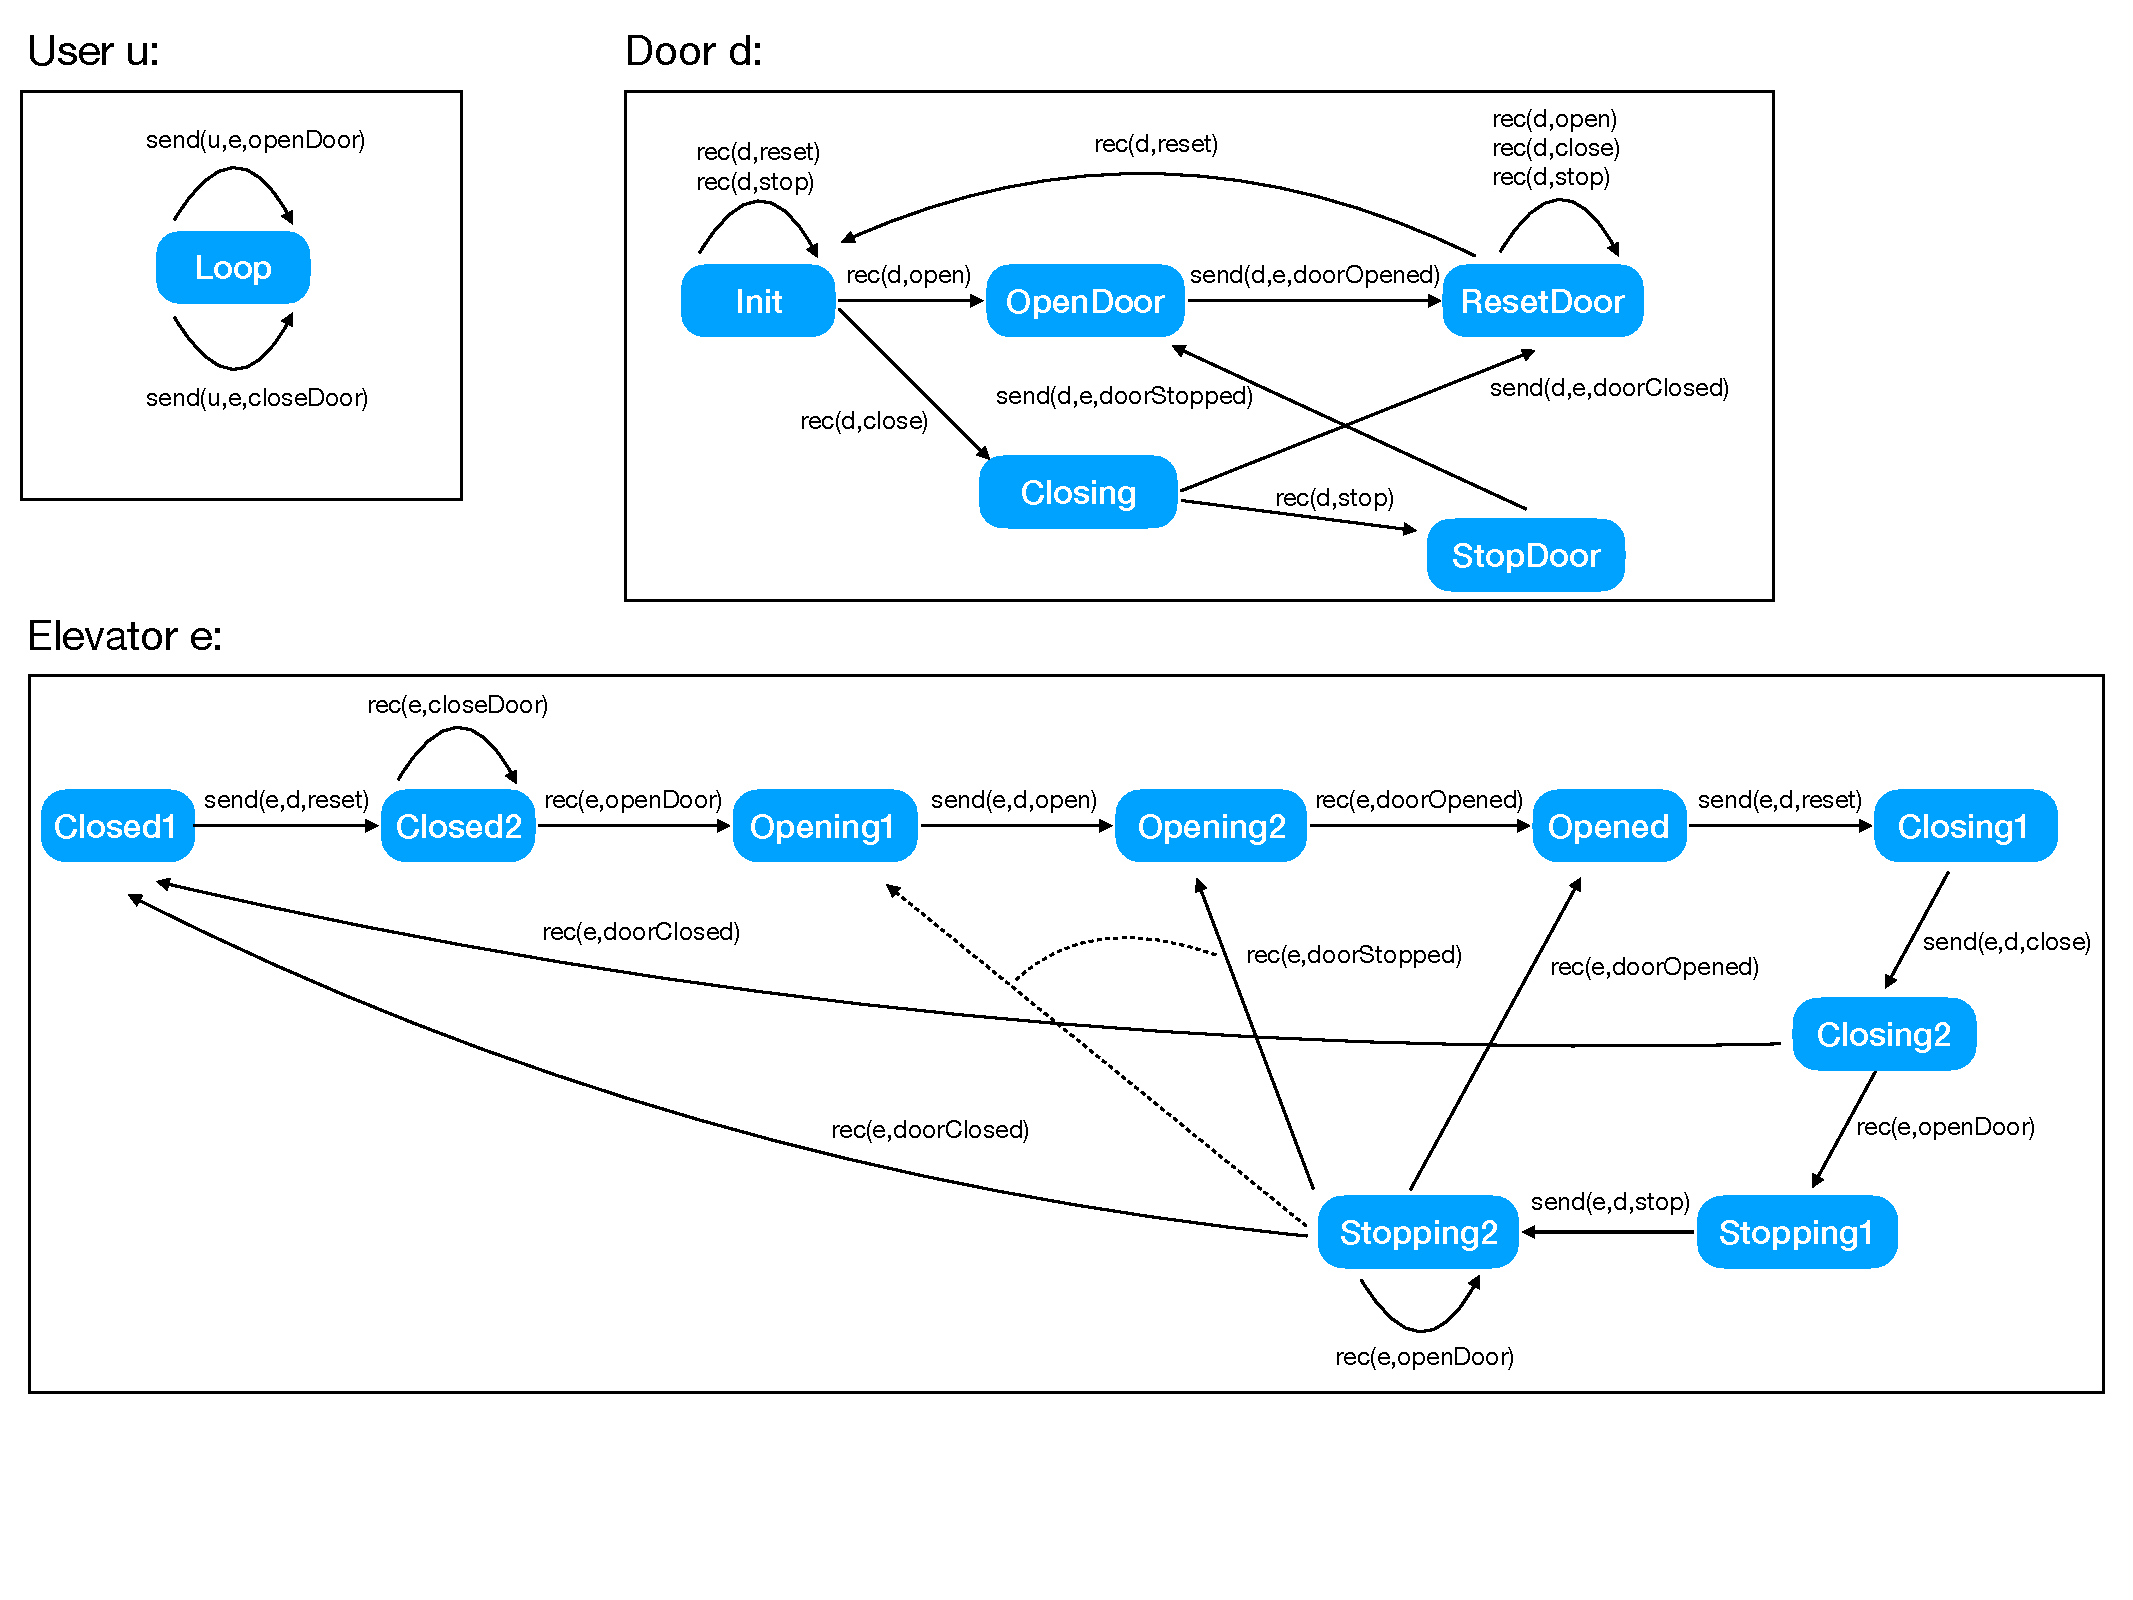
\includegraphics[width=13cm]{elevator.pdf}
%\caption{The Elevator example}
%\label{fig:elevator}
%\end{figure}
%
%\begin{figure}
%\begin{subfigure}[t]{6cm}
%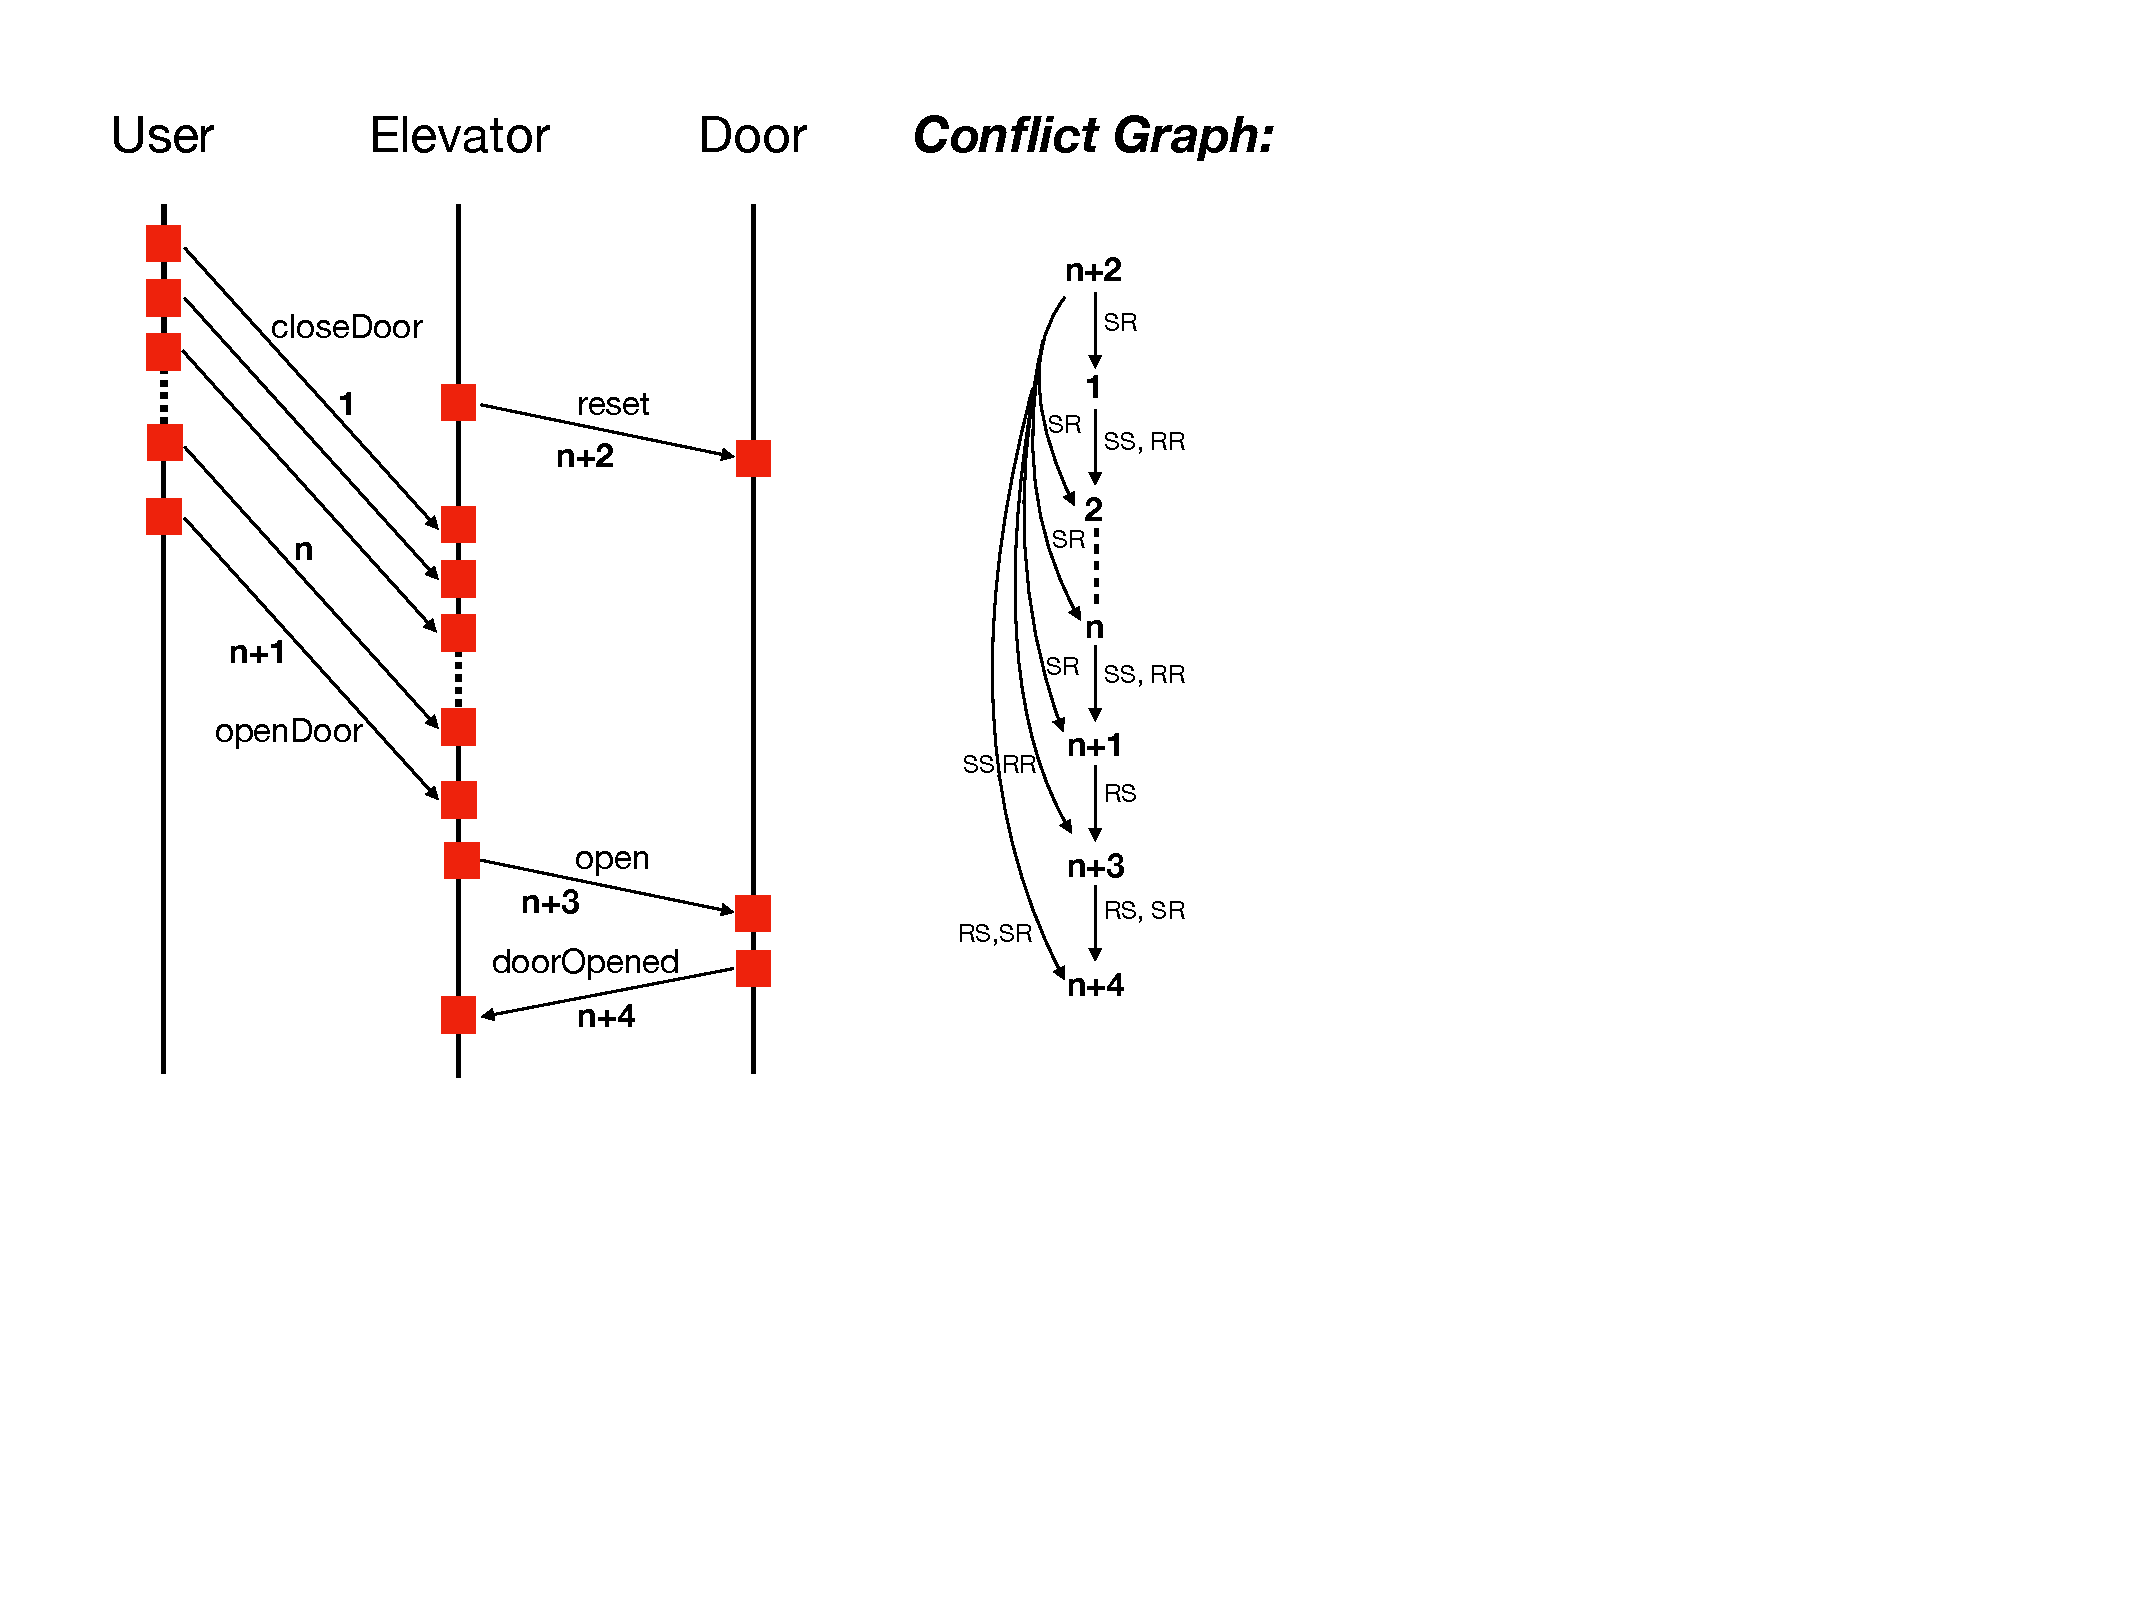
\includegraphics[width=6cm]{MSC-elevator1.pdf}
%\caption{A synchronizable execution.}
%\label{fig:elevator-exec1}
%\end{subfigure}
%\hspace{1cm}
%\begin{subfigure}[t]{5cm}
%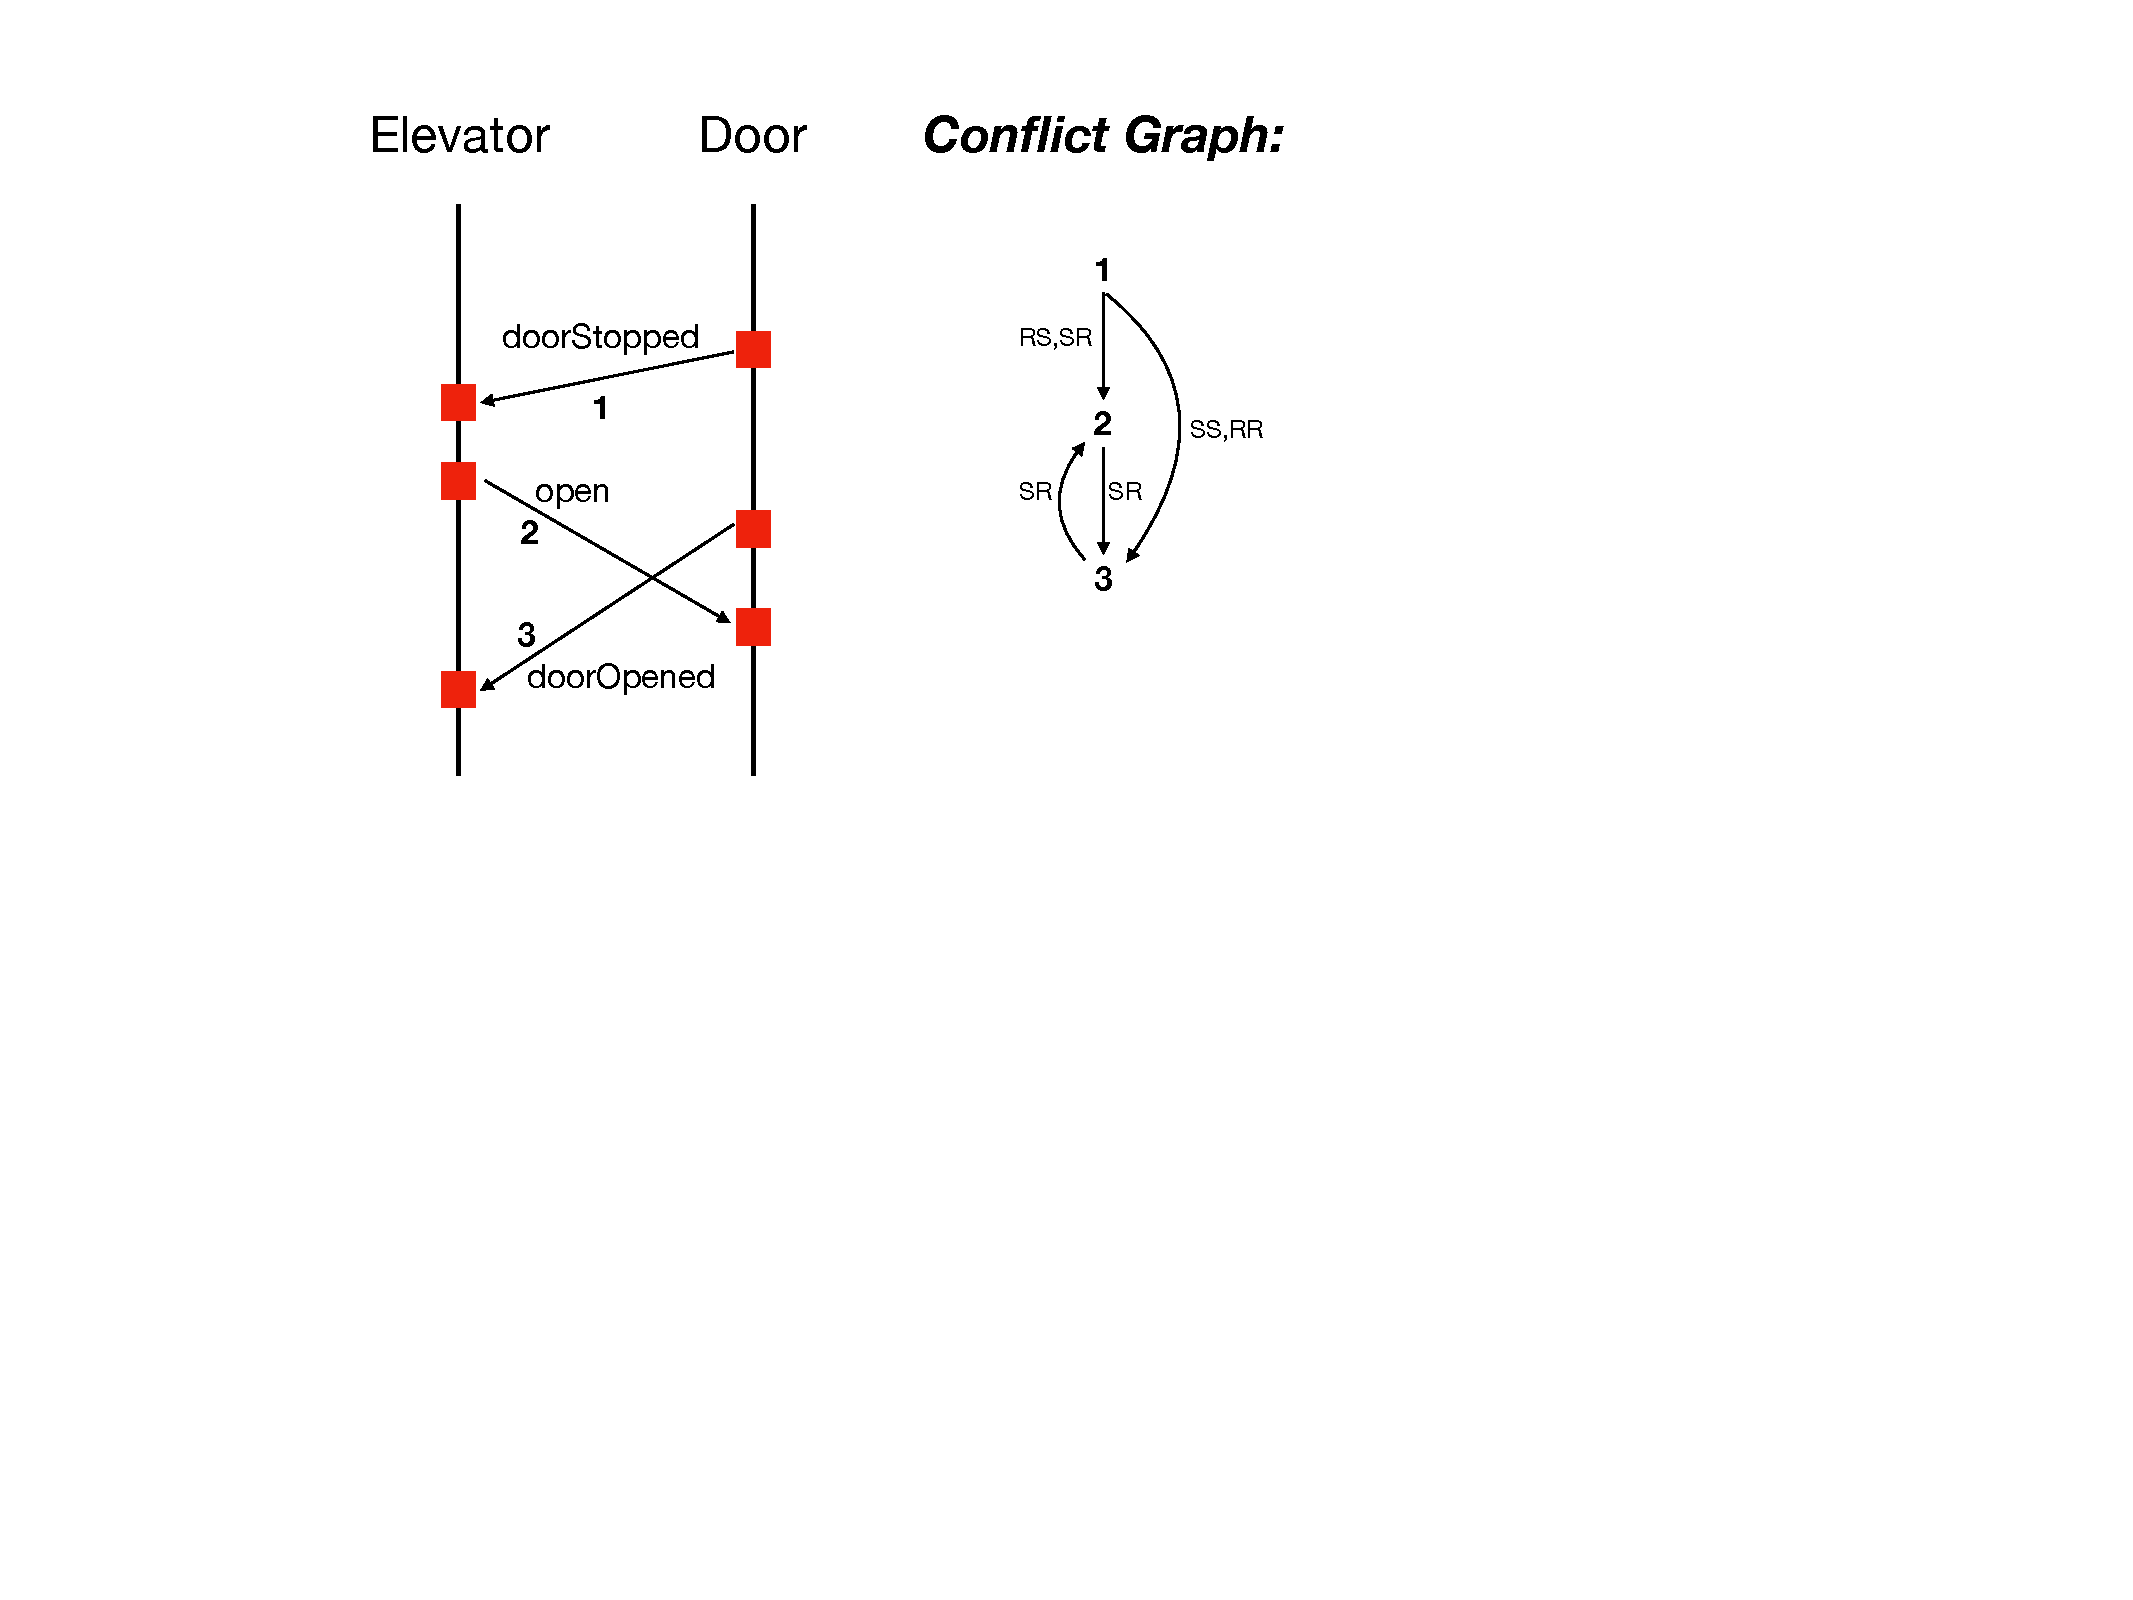
\includegraphics[width=5cm]{MSC-elevator2.pdf}
%\caption{A computation with a 2-exchange.}
%\label{fig:elevator-exec2}
%\end{subfigure}
%\caption{Executions of the elevator.}
%\label{fig:elevator-exec}
%\end{figure}

\begin{figure}[t]
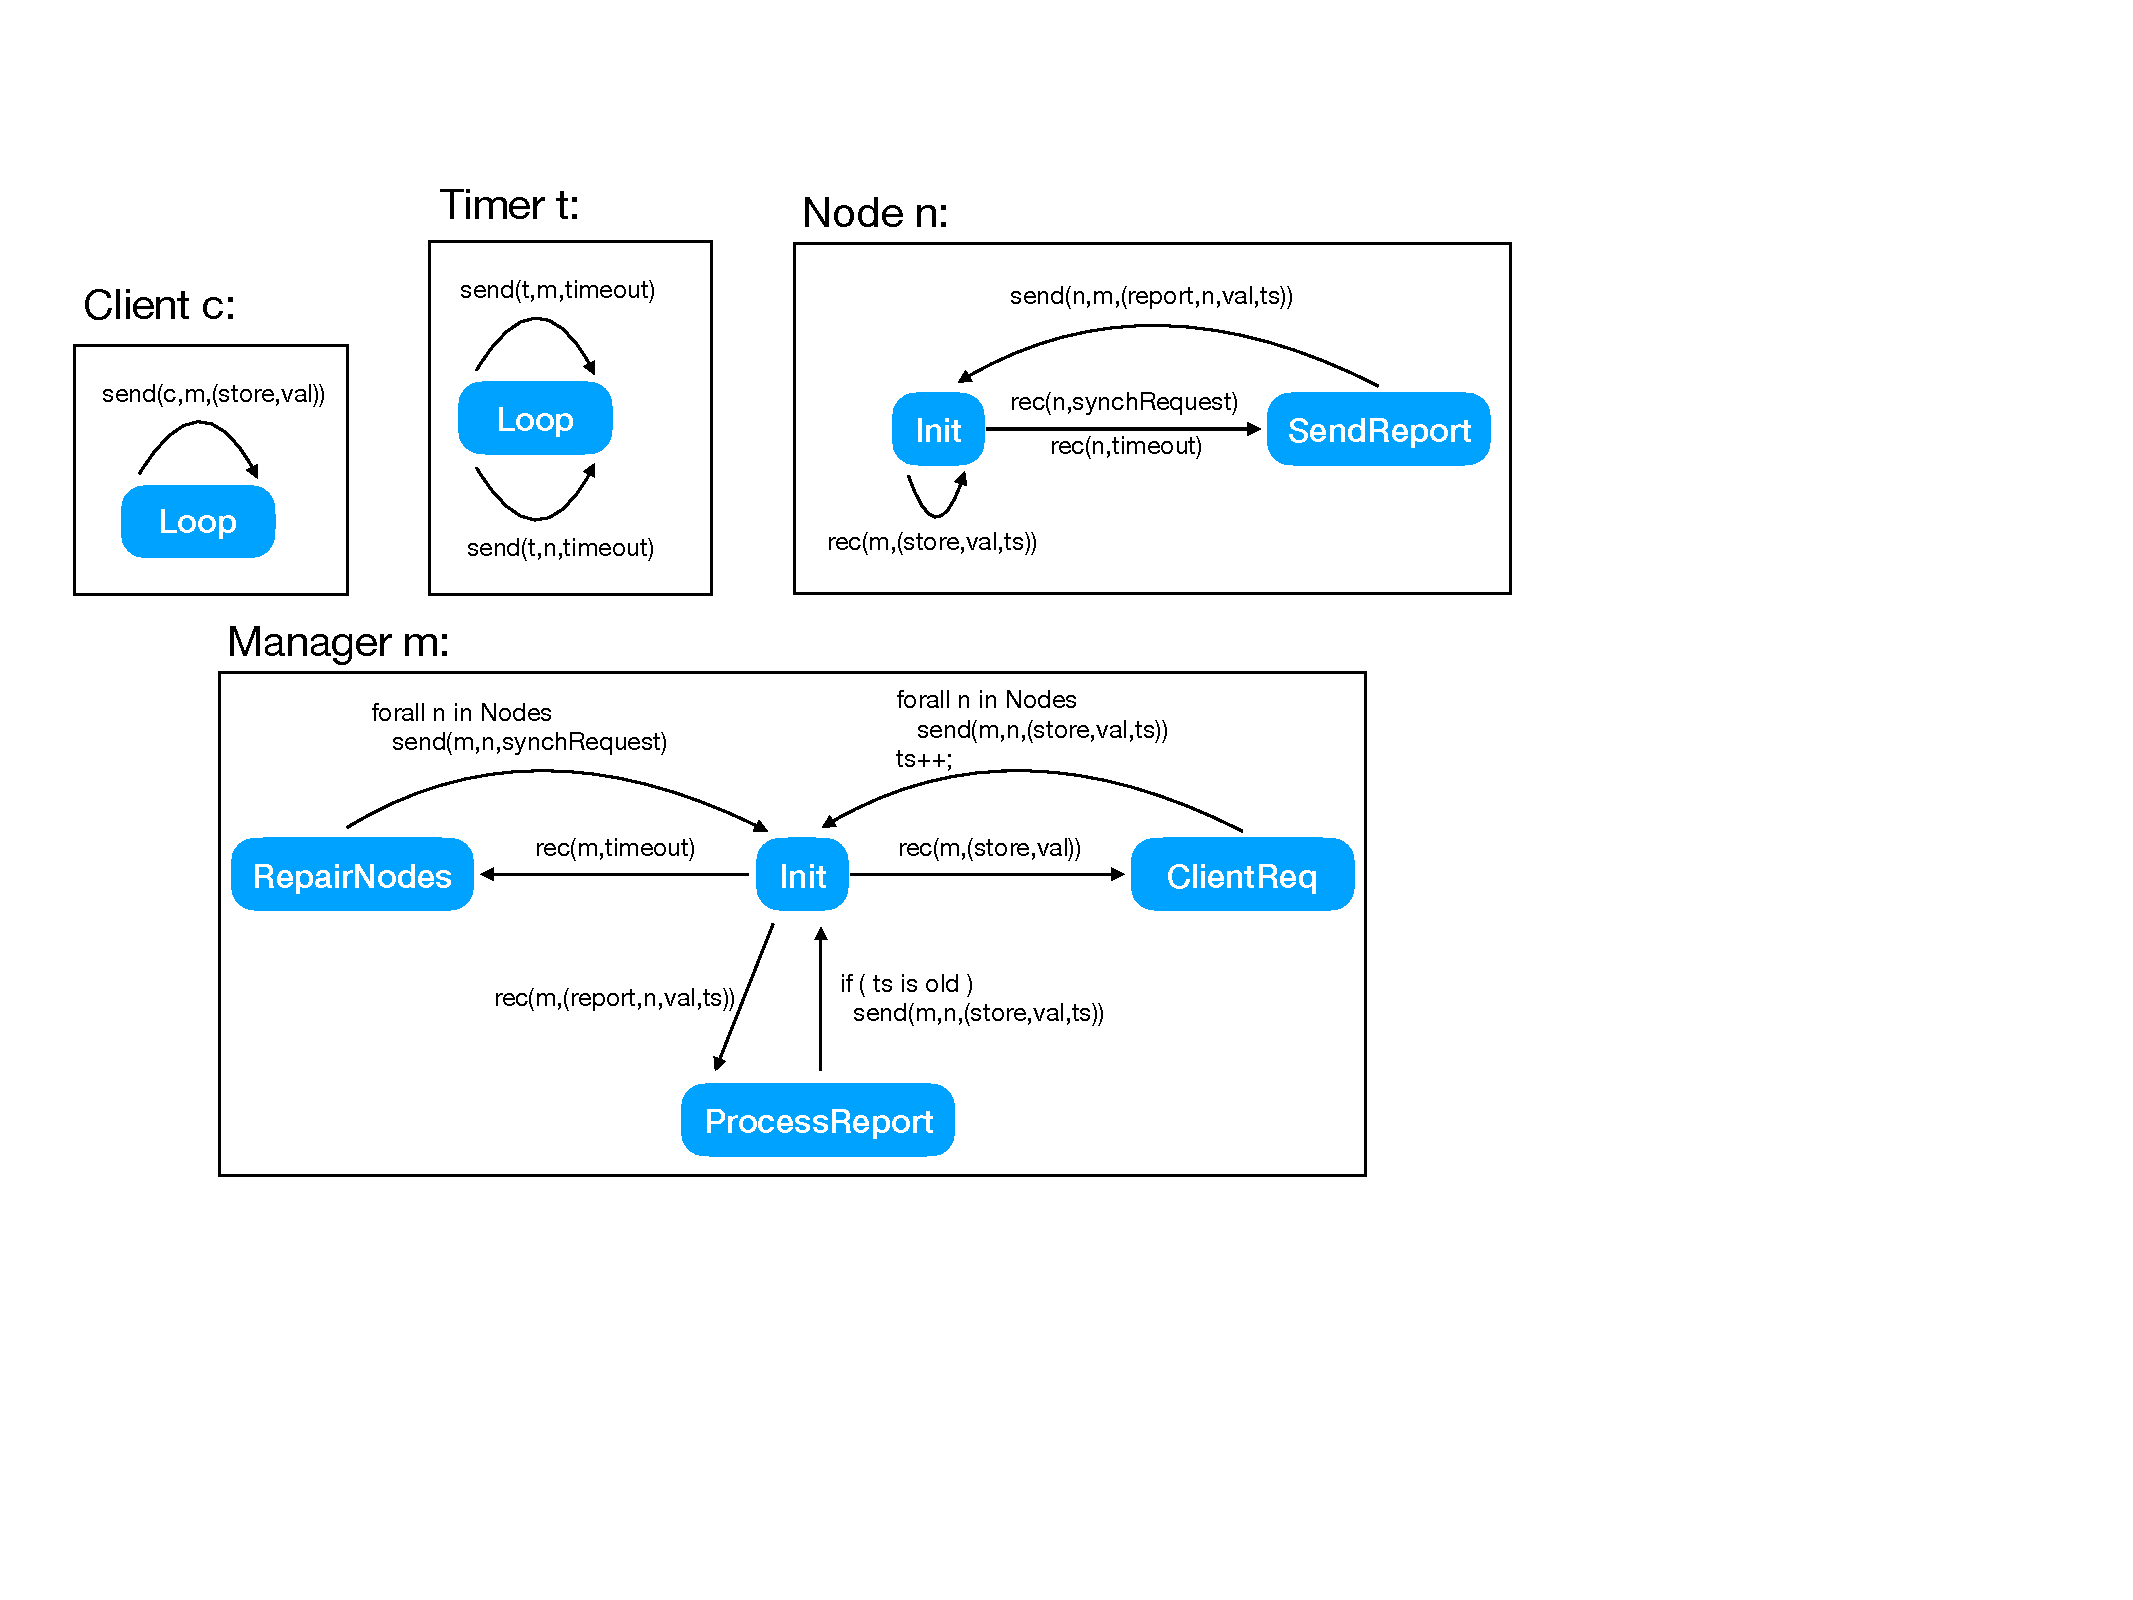
\includegraphics[width=10cm]{replication.pdf}
\caption{A replication storage protocol.}
\label{fig:replication}
\end{figure}

\begin{figure}[t]
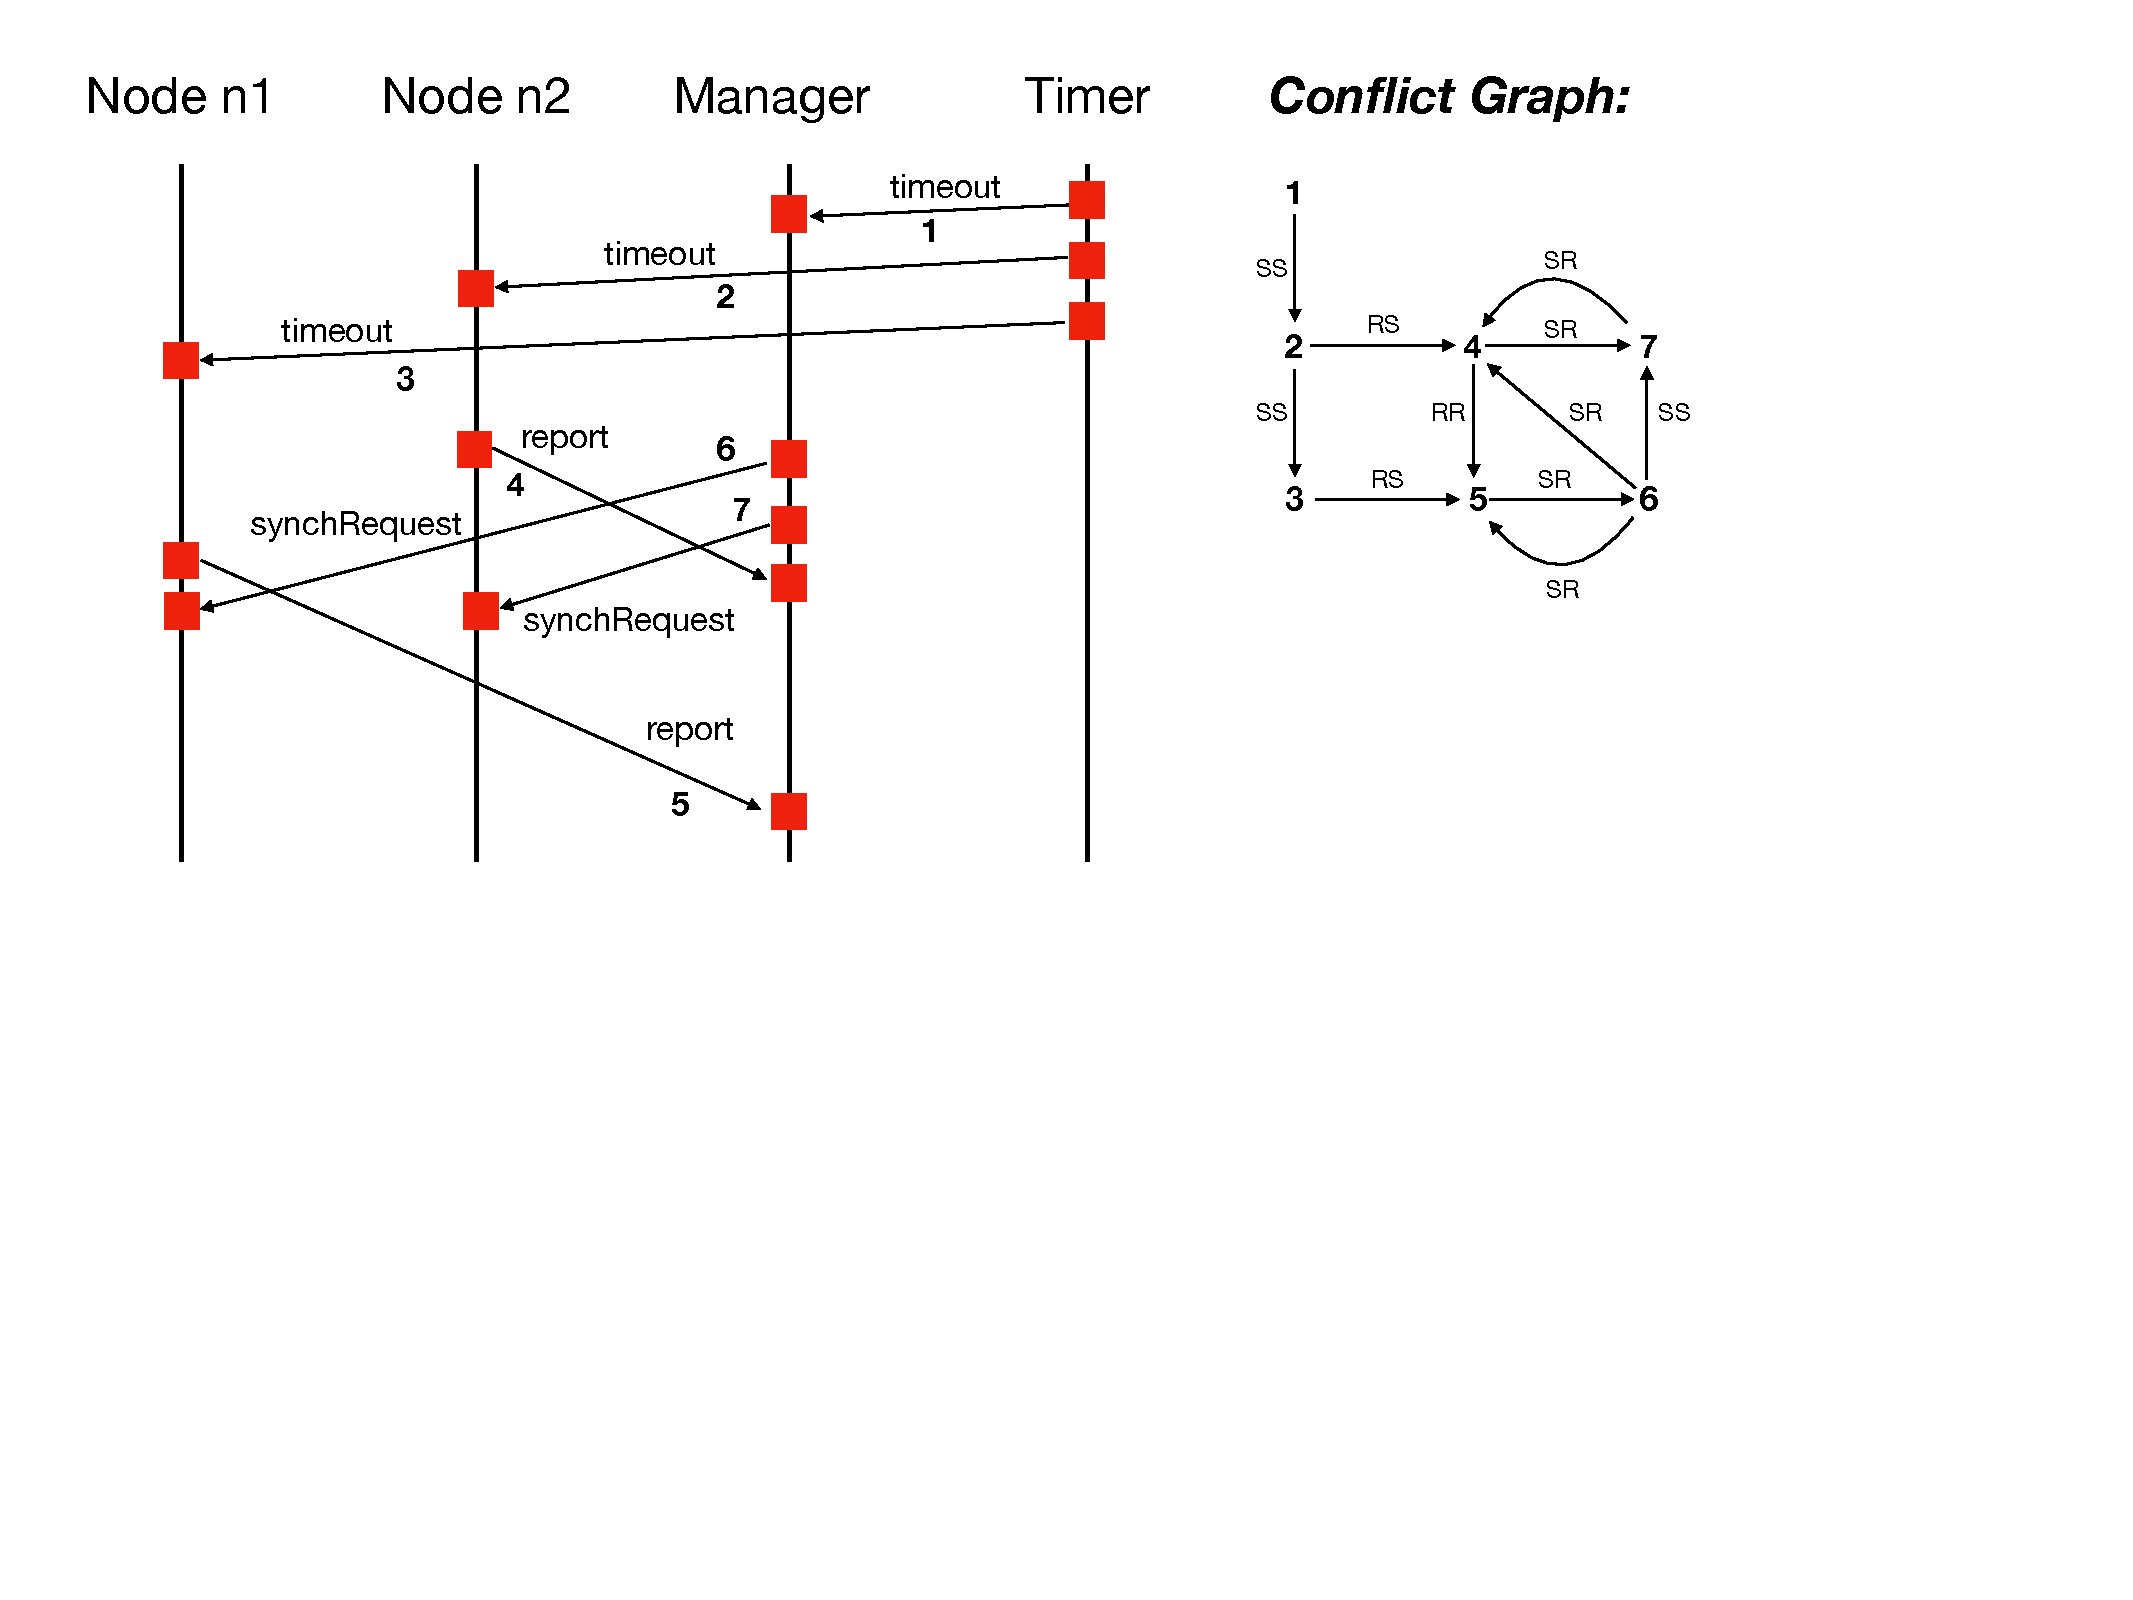
\includegraphics[width=7cm]{MSC-storage.pdf}
\caption{An execution of the replication storage protocol and its conflict graph.}
\label{fig:replic-exec}
\end{figure}
